% =============================================================================
% APPENDIX BM: METHOD-PAPERINT: Paper Integration Methodology
% =============================================================================
% Module: BCM2_METHOD_PAPERINT
% Version: 1.0 (January 2026)
% Status: Final
% Category: METHOD (Methodology)
% Language: English
%
% PURPOSE: This appendix documents the standardized workflow for integrating
% scientific papers into the EBF framework, including the 2D classification
% system (Content Level x Integration Level) and the Learning Loop mechanism.
%
% =============================================================================

% =============================================================================
% CROSS-REFERENCE STRUCTURE
% =============================================================================
%
% CHAPTER LINKAGE:
% - Primary Chapter: All chapters (paper integration affects all)
% - Primary Section: CLAUDE.md §Paper Integration Workflow
% - Secondary: Ch. 11 (§11.3 Motivated vs Informed Beliefs - citation example)
%
% This appendix provides methodology for Chapter--Paper linkages throughout EBF.
%
% SSOT (Single Source of Truth) ARCHITECTURE:
% This appendix (BM) is the PRIMARY SSOT for the 2D Classification System.
% The following files implement and track the system:
%
% | Priority | File                                      | Purpose                    |
% |----------|-------------------------------------------|----------------------------|
% | 1        | THIS APPENDIX (BM)                        | Formal definitions, axioms |
% | 2        | data/paper-integration-metrics.yaml       | Workflow timing metrics    |
% | 3        | data/paper-integration-learnings.yaml     | Learning database          |
% | 4        | data/paper-integration-queue.yaml         | Papers to upgrade          |
% | 5        | docs/frameworks/paper-database-quality-dimensions.md | Summary (markdown) |
%
% DEPENDENCIES (what this appendix REQUIRES):
% - Appendix GLS: Glossary definitions
% - bcm_master.bib: Master bibliography
% - data/paper-integration-metrics.yaml: Workflow metrics database
% - data/paper-integration-learnings.yaml: Learning database
% - data/paper-integration-queue.yaml: Upgrade queue
%
% DEPENDENTS (what REQUIRES this appendix):
% - All LIT-* appendices (Literature reviews)
% - All chapters with paper citations
% - /upgrade-paper skill
% - docs/frameworks/paper-database-quality-dimensions.md (summary)
%
% =============================================================================

\chapter{METHOD-PAPERINT: Paper Integration Methodology}
\label{app:method-paperint}

%%%%%%%%%%%%%%%%%%%%%%%%%%%%%%%%%%%%%%%%%%%%%%%%%%%%%%%%%%%%%%%%%%%%%%%%%%%%%%%
% ABSTRACT
%%%%%%%%%%%%%%%%%%%%%%%%%%%%%%%%%%%%%%%%%%%%%%%%%%%%%%%%%%%%%%%%%%%%%%%%%%%%%%%

\begin{abstract}
This appendix documents the standardized methodology for integrating scientific
papers into the Evidence-Based Framework (EBF). The core contribution is a
\textbf{2D Classification System} that independently tracks content depth
(Content Levels 0--3) and framework integration depth (Integration Levels 1--5).
A \textbf{Learning Loop} mechanism ensures continuous improvement by documenting
lessons learned from each integration session. The methodology enables systematic,
reproducible paper integration with clear quality thresholds and validation criteria.
\end{abstract}

%%%%%%%%%%%%%%%%%%%%%%%%%%%%%%%%%%%%%%%%%%%%%%%%%%%%%%%%%%%%%%%%%%%%%%%%%%%%%%%
% QUICK REFERENCE BOX
%%%%%%%%%%%%%%%%%%%%%%%%%%%%%%%%%%%%%%%%%%%%%%%%%%%%%%%%%%%%%%%%%%%%%%%%%%%%%%%

\begin{tcolorbox}[colback=blue!5!white, colframe=blue!75!black,
    title=Quick Reference: Paper Integration (MECE-Compliant)]

\textbf{Workflow Overview:}
\begin{enumerate}[nosep]
    \item \textbf{Ersterfassung} (Section~\ref{sec:paperint-ersterfassung}): YAML + BibTeX $\rightarrow$ $(L1, I1)$
    \item \textbf{Upgrade} (Section~\ref{sec:paperint-upgrade}): $(L1, I1) \rightarrow \ldots \rightarrow (L3, I5)$
\end{enumerate}

\vspace{0.3em}
\textbf{2D Classification System (Orthogonal by Design):}

\begin{tabular}{@{}p{4.5cm}|p{5.5cm}@{}}
\textbf{Content Level (Structural)} & \textbf{Integration Level (EBF-Specific)} \\
\midrule
L0 = Metadata only & I1 = Classified (\texttt{use\_for}, \texttt{evidence\_tier}) \\
L1 = + Research Question ($S_1$) & I2 = Theorized (+ \texttt{theory\_support}) \\
L2 = + Method, Sample, Findings ($S_{1-4}$) & I3 = Exemplified (+ CAS-XXX) \\
L3 = + Validity, Reproducibility ($S_{1-6}$) & I4 = Parameterized (+ PAR-XXX) \\
 & I5 = Canonized (+ Appendix + Chapter) \\
\end{tabular}

\vspace{0.3em}
\textbf{MECE Rule:} Content = structural completeness | Integration = EBF linkages

\textbf{Key Insight:} Structure determines level, not character count

\textbf{Skill:} \texttt{/upgrade-paper PAP-xxx}

\textbf{SSOT Data Files:}
\begin{itemize}[nosep]
    \item \texttt{data/paper-integration-metrics.yaml} -- Workflow timing
    \item \texttt{data/paper-integration-learnings.yaml} -- Learning database
    \item \texttt{data/paper-integration-queue.yaml} -- Upgrade queue
\end{itemize}

\end{tcolorbox}

%%%%%%%%%%%%%%%%%%%%%%%%%%%%%%%%%%%%%%%%%%%%%%%%%%%%%%%%%%%%%%%%%%%%%%%%%%%%%%%
% SSOT BOX
%%%%%%%%%%%%%%%%%%%%%%%%%%%%%%%%%%%%%%%%%%%%%%%%%%%%%%%%%%%%%%%%%%%%%%%%%%%%%%%

\begin{tcolorbox}[colback=red!5!white, colframe=red!75!black,
    title=\textbf{SSOT: Single Source of Truth Hierarchy}]

This appendix (BM) defines the \textbf{formal 2D Classification System}.
The following files track and implement the system:

\begin{table}[H]
\centering
\begin{tabular}{@{}clp{6cm}@{}}
\toprule
\textbf{Priority} & \textbf{File} & \textbf{Purpose} \\
\midrule
1 & This Appendix (BM) & Formal definitions (L0--L3 $\times$ 1--5) \\
2 & \texttt{paper-integration-metrics.yaml} & Per-paper workflow metrics \\
3 & \texttt{paper-integration-learnings.yaml} & Error patterns, lessons learned \\
4 & \texttt{paper-integration-queue.yaml} & Papers pending upgrade \\
5 & \texttt{paper-database-quality-*.md} & Markdown summary \\
\bottomrule
\end{tabular}
\end{table}

\textbf{Rule:} When definitions conflict, higher-priority sources are authoritative.

\end{tcolorbox}

%%%%%%%%%%%%%%%%%%%%%%%%%%%%%%%%%%%%%%%%%%%%%%%%%%%%%%%%%%%%%%%%%%%%%%%%%%%%%%%
% SSOT DATA ARCHITECTURE BOX
%%%%%%%%%%%%%%%%%%%%%%%%%%%%%%%%%%%%%%%%%%%%%%%%%%%%%%%%%%%%%%%%%%%%%%%%%%%%%%%

\begin{tcolorbox}[colback=green!5!white, colframe=green!75!black,
    title=\textbf{SSOT Data Architecture: Paper Database}]

The paper database follows a strict \textbf{Single Source of Truth (SSOT)} architecture
with three layers:

\begin{table}[H]
\centering
\begin{tabular}{@{}clp{5.5cm}@{}}
\toprule
\textbf{Layer} & \textbf{Location} & \textbf{Content} \\
\midrule
\textbf{PRIMÄR} & \texttt{data/paper-references/PAP-\{key\}.yaml} &
    All metadata + EBF fields + Prior Score \\
\textbf{FULL-TEXT} & \texttt{data/paper-texts/PAP-\{key\}.md} &
    Complete paper text (L1--L3 content) \\
\textbf{GENERATED} & \texttt{bibliography/bcm\_master.bib} &
    BibTeX for LaTeX (generated from YAML) \\
\bottomrule
\end{tabular}
\end{table}

\textbf{YAML Schema (PRIMÄR):}
\begin{verbatim}
superkey: PAP-fehr1999theory
title: "A Theory of Fairness..."
author: "Fehr, Ernst and Schmidt, Klaus M"
year: 1999
doi: "10.1162/003355399556151"
# Publication Type (Definition 0)
publication_type:
  type: ART              # {ART, BOOK, CHAP, CONF, WP, REP, THESIS}
  venue: journal         # Venue class V
  review_status: 2       # R: 0=none, 1=editorial, 2=peer
  empirical_content: 1   # E: 0=theoretical, 1=mixed, 2=empirical
  originality: primary   # O: {primary, replication, review, meta}
  journal_tier: top      # J in J_top => Tier 1
# EBF Integration (Definition 3-4)
ebf_integration:
  evidence_tier: 1       # Derived from publication_type
  use_for: [CORE-WHAT, LIT-FEH, parameter]
  theory_support: MS-SP-001
  parameter: "alpha = 0.85, beta = 0.315"
# Content Level (Definition 2)
full_text:
  available: true
  path: "data/paper-texts/PAP-fehr1999theory.md"
  content_level: L2
  character_count: 9958
# L1/L2 Template (Definition 2a) - if no full_text
summary:
  abstract_extended: "Extended abstract..."
  key_findings: "1. Finding A\n2. Finding B"
  ebf_relevance: "10C: WHAT, HOW; Theory: MS-SP-001"
  sources: "https://..."
  template_source: "papers/evaluated/integrated/..."
  migrated_date: "2026-02-01"
# Prior Score (Theorem 2)
prior_score:
  prior_score: 0.456
  classification: MINIMAL
  confidence_multiplier: 0.95   # L2 = 0.95
\end{verbatim}

\textbf{Scripts:}
\begin{itemize}[nosep]
    \item \texttt{scripts/migrate\_bibtex\_to\_yaml.py} -- Migrate EBF fields to YAML
    \item \texttt{scripts/integrate\_l1l2\_templates.py} -- Migrate L1/L2 templates to YAML \texttt{summary}
    \item \texttt{scripts/compute\_prior\_scores.py} -- Compute $\pi(p)$ for all papers
    \item \texttt{scripts/generate\_bibtex\_from\_yaml.py} -- Generate BibTeX (planned)
\end{itemize}

\textbf{Data Flow:}
\begin{equation}
\text{YAML (source)} \xrightarrow{\text{generate}} \text{BibTeX (output)} \xrightarrow{\text{compile}} \text{LaTeX PDF}
\end{equation}

\end{tcolorbox}

%%%%%%%%%%%%%%%%%%%%%%%%%%%%%%%%%%%%%%%%%%%%%%%%%%%%%%%%%%%%%%%%%%%%%%%%%%%%%%%
% APPENDIX SCOPE BOX
%%%%%%%%%%%%%%%%%%%%%%%%%%%%%%%%%%%%%%%%%%%%%%%%%%%%%%%%%%%%%%%%%%%%%%%%%%%%%%%

\begin{tcolorbox}[
    colback=orange!5!white,
    colframe=orange!75!black,
    title={\textbf{Appendix Scope: Ziel / In-Scope / Out-of-Scope}},
    fonttitle=\bfseries
]

\textbf{Ziel (Objective):}
Standardize paper integration workflow with reproducible quality criteria and
continuous learning mechanism.

\vspace{0.3cm}
\textbf{In-Scope:}
\begin{itemize}[nosep]
    \item 2D Classification System (Content Level $\times$ Integration Level)
    \item Step-by-step upgrade workflow
    \item Learning Loop mechanism
    \item Validation criteria and thresholds
    \item Common error patterns and prevention
\end{itemize}

\vspace{0.3cm}
\textbf{Out-of-Scope (delegated):}
\begin{itemize}[nosep]
    \item LIT-Appendix content $\rightarrow$ Individual LIT-* appendices
    \item BibTeX syntax $\rightarrow$ Standard LaTeX documentation
    \item Case Registry schema $\rightarrow$ Appendix CAS
    \item Theory Catalog schema $\rightarrow$ Appendix MS
\end{itemize}

\end{tcolorbox}

%%%%%%%%%%%%%%%%%%%%%%%%%%%%%%%%%%%%%%%%%%%%%%%%%%%%%%%%%%%%%%%%%%%%%%%%%%%%%%%
% SECTION 1: THE 2D CLASSIFICATION SYSTEM
%%%%%%%%%%%%%%%%%%%%%%%%%%%%%%%%%%%%%%%%%%%%%%%%%%%%%%%%%%%%%%%%%%%%%%%%%%%%%%%

\section{The 2D Classification System}
\label{sec:paperint-2d-system}

Papers in EBF are classified along two orthogonal dimensions.

%%%%%%%%%%%%%%%%%%%%%%%%%%%%%%%%%%%%%%%%%%%%%%%%%%%%%%%%%%%%%%%%%%%%%%%%%%%%%%%
% PUBLICATION TYPE TAXONOMY
%%%%%%%%%%%%%%%%%%%%%%%%%%%%%%%%%%%%%%%%%%%%%%%%%%%%%%%%%%%%%%%%%%%%%%%%%%%%%%%

\subsection{Publication Type Taxonomy (Prerequisite)}
\label{sec:paperint-pubtype}

Before classifying content and integration levels, we must formally define
\textbf{what constitutes a ``paper''} in the EBF bibliography. This taxonomy
is \textbf{not based on character count} but on structural properties.

\begin{tcolorbox}[colback=blue!5!white, colframe=blue!75!black,
    title=\textbf{Definition 0: Publication Type Space $\mathcal{T}$}]

Let $\mathcal{D}$ denote the set of all documents. We define the \textbf{Publication Type}
as a function $T: \mathcal{D} \to \mathcal{T}$ based on four orthogonal dimensions:

\textbf{Dimension 1: Venue Class $\mathcal{V}$}
\begin{equation}
\mathcal{V} = \{\texttt{journal}, \texttt{book}, \texttt{chapter}, \texttt{conference}, \texttt{working}, \texttt{report}, \texttt{thesis}, \texttt{preprint}\}
\end{equation}

\textbf{Dimension 2: Review Status $R \in \{0, 1, 2\}$}
\begin{equation}
R(d) = \begin{cases}
0 & \text{no formal review (preprint, working paper)} \\
1 & \text{editorial review (book chapter, report)} \\
2 & \text{peer review (journal, conference proceedings)}
\end{cases}
\end{equation}

\textbf{Dimension 3: Empirical Content $E \in \{0, 1, 2\}$}
\begin{equation}
E(d) = \begin{cases}
0 & \text{purely theoretical (proofs, models)} \\
1 & \text{mixed (theory + data)} \\
2 & \text{purely empirical (experiments, surveys)}
\end{cases}
\end{equation}

\textbf{Dimension 4: Originality $O$}
\begin{equation}
O = \{\texttt{primary}, \texttt{replication}, \texttt{review}, \texttt{meta}, \texttt{commentary}\}
\end{equation}

\end{tcolorbox}

\begin{tcolorbox}[colback=blue!5!white, colframe=blue!75!black,
    title=\textbf{Definition 0a: Canonical Publication Types (MECE Partition)}]

The EBF bibliography partitions $\mathcal{D}$ into seven \textbf{mutually exclusive} types:

\begin{table}[H]
\centering
\begin{tabular}{@{}llcccp{4cm}@{}}
\toprule
\textbf{Type} & \textbf{Code} & $R$ & $\mathcal{V}$ & \textbf{Formal Criterion} \\
\midrule
Journal Article & \texttt{ART} & $=2$ & journal & $R=2 \land V=\texttt{journal}$ \\
Book & \texttt{BOOK} & $\geq 1$ & book & $V=\texttt{book} \land \neg\exists$ parent \\
Book Chapter & \texttt{CHAP} & $\geq 1$ & chapter & $V=\texttt{chapter} \land \exists$ parent \\
Conference Paper & \texttt{CONF} & $=2$ & conference & $R=2 \land V=\texttt{conference}$ \\
Working Paper & \texttt{WP} & $=0$ & working & $R=0 \land V \in \{\texttt{working}, \texttt{preprint}\}$ \\
Report & \texttt{REP} & $\leq 1$ & report & $V=\texttt{report}$ \\
Thesis & \texttt{THESIS} & $=2$ & thesis & $V=\texttt{thesis}$ (committee review) \\
\bottomrule
\end{tabular}
\end{table}

\textbf{MECE Verification:}
\begin{itemize}[nosep]
    \item \textbf{Mutually Exclusive:} Each document maps to exactly one type
    \item \textbf{Collectively Exhaustive:} $\bigcup_{t \in \mathcal{T}} t = \mathcal{D}$
\end{itemize}

\end{tcolorbox}

\begin{tcolorbox}[colback=blue!5!white, colframe=blue!75!black,
    title=\textbf{Definition 0b: Evidence Tier Derivation from Publication Type}]

The \textbf{Evidence Tier} $\tau(d)$ is \textbf{formally derived} from Publication Type:

\begin{equation}
\tau(d) = \begin{cases}
1.0 \text{ (Tier 1)} & \text{if } T(d) \in \{\texttt{ART}, \texttt{CONF}\} \land J(d) \in \mathcal{J}_{\text{top}} \\
0.8 \text{ (Tier 2)} & \text{if } T(d) \in \{\texttt{ART}, \texttt{CONF}, \texttt{BOOK}\} \land R(d) = 2 \\
0.5 \text{ (Tier 3)} & \text{if } T(d) \in \{\texttt{WP}, \texttt{REP}, \texttt{CHAP}\} \lor R(d) < 2
\end{cases}
\end{equation}

Where $\mathcal{J}_{\text{top}}$ is the set of top-tier journals:
\begin{equation}
\mathcal{J}_{\text{top}} = \{\text{QJE}, \text{AER}, \text{Econometrica}, \text{JPE}, \text{REStud}, \text{Science}, \text{Nature}, ...\}
\end{equation}

\textbf{Key Insight:} Evidence Tier is \textbf{not arbitrary} but follows from:
\begin{enumerate}[nosep]
    \item Review rigor ($R$)
    \item Journal prestige ($J \in \mathcal{J}_{\text{top}}$)
    \item Publication finality ($\texttt{WP} \to \texttt{ART}$ upgrade path)
\end{enumerate}

\end{tcolorbox}

\begin{tcolorbox}[colback=green!5!white, colframe=green!75!black,
    title=\textbf{Axiom PUB-1: Publication Type Immutability}]

Once assigned, the Publication Type $T(d)$ is \textbf{immutable} unless:
\begin{enumerate}[nosep]
    \item A Working Paper is published $\Rightarrow$ $T: \texttt{WP} \to \texttt{ART}$
    \item A Preprint is accepted $\Rightarrow$ $T: \texttt{WP} \to \texttt{ART}$ or $\texttt{CONF}$
\end{enumerate}

In such cases, the \textbf{published version supersedes} the working paper,
and the old entry is marked as \texttt{superseded\_by: PAP-newkey}.

\end{tcolorbox}

\begin{tcolorbox}[colback=green!5!white, colframe=green!75!black,
    title=\textbf{Axiom PUB-2: Type-Content Independence}]

Publication Type $T(d)$ and Content Level $C(d)$ are \textbf{orthogonal}:

\begin{equation}
T(d) \perp C(d)
\end{equation}

A Working Paper can have $C = L3$ (full text), and a Journal Article can have $C = L0$ (metadata only).
The 2D Classification $(C, I)$ operates \textbf{within} each Publication Type.

\end{tcolorbox}

%%%%%%%%%%%%%%%%%%%%%%%%%%%%%%%%%%%%%%%%%%%%%%%%%%%%%%%%%%%%%%%%%%%%%%%%%%%%%%%
% FORMAL DEFINITIONS (Content & Integration)
%%%%%%%%%%%%%%%%%%%%%%%%%%%%%%%%%%%%%%%%%%%%%%%%%%%%%%%%%%%%%%%%%%%%%%%%%%%%%%%

\subsection{Formal Mathematical Definitions}
\label{sec:paperint-formal}

Let $\mathcal{P}$ denote the set of all papers in the EBF bibliography.

\begin{tcolorbox}[colback=blue!5!white, colframe=blue!75!black,
    title=\textbf{Definition 1: Field Sets (Semantic Partition)}]

\textbf{Content Fields} (paper-internal information):
\begin{equation}
\mathcal{F}_C = \{\texttt{abstract}, \texttt{keywords}, \texttt{methodology}, \texttt{sample}, \texttt{findings}, \texttt{limitations}, \texttt{full\_text}, \texttt{paper\_bib}\}
\end{equation}

\textbf{Integration Fields} (EBF-specific linkages):
\begin{equation}
\mathcal{F}_I = \{\texttt{use\_for}, \texttt{evidence\_tier}, \texttt{theory\_support}, \texttt{case\_links}, \texttt{parameter}, \texttt{appendix\_refs}, \texttt{chapter\_refs}\}
\end{equation}

\textbf{MECE Constraint:}
\begin{equation}
\mathcal{F}_C \cap \mathcal{F}_I = \emptyset \quad \text{(Mutually Exclusive)}
\end{equation}

\end{tcolorbox}

\begin{tcolorbox}[colback=blue!5!white, colframe=blue!75!black,
    title=\textbf{Definition 2: Content Level Function $C: \mathcal{P} \to \{L0, L1, L2, L3\}$}]

Content Level is determined by \textbf{structural completeness}, not character count.
Let $\phi_S(p)$ denote the set of documented structural characteristics for paper $p$.

\textbf{The 6 Structural Characteristics $\mathcal{S}$:}
\begin{table}[H]
\centering
\begin{tabular}{@{}clp{6cm}@{}}
\toprule
\textbf{ID} & \textbf{Characteristic} & \textbf{Content} \\
\midrule
$S_1$ & Research Question & Hypothesis, 10C mapping \\
$S_2$ & Methodology & Design, instrument, identification \\
$S_3$ & Sample/Data & N, population, sampling, representativeness \\
$S_4$ & Findings & Coefficients, effect sizes, robustness \\
$S_5$ & Validity & Internal, external, limitations \\
$S_6$ & Reproducibility & Data/code availability, replication status \\
\bottomrule
\end{tabular}
\end{table}

\textbf{Content Level Assignment:}
\begin{equation}
C(p) =
\begin{cases}
L0 & \text{if } |\phi_S(p)| = 0 \quad \text{(metadata only)} \\
L1 & \text{if } S_1 \in \phi_S(p) \quad \text{(research question known)} \\
L2 & \text{if } \{S_1, S_2, S_3, S_4\} \subseteq \phi_S(p) \quad \text{(study evaluable)} \\
L3 & \text{if } \{S_1, S_2, S_3, S_4, S_5, S_6\} \subseteq \phi_S(p) \lor \texttt{full\_text} = \text{true}
\end{cases}
\end{equation}

\textbf{Key Insight:} A 2-page summary with complete $S_1$--$S_4$ is $L2$.
A 100-page document without methodology is $L1$. Structure determines level, not length.

\end{tcolorbox}

%%%%%%%%%%%%%%%%%%%%%%%%%%%%%%%%%%%%%%%%%%%%%%%%%%%%%%%%%%%%%%%%%%%%%%%%%%%%%%%
% L1/L2 TEMPLATE DEFINITION
%%%%%%%%%%%%%%%%%%%%%%%%%%%%%%%%%%%%%%%%%%%%%%%%%%%%%%%%%%%%%%%%%%%%%%%%%%%%%%%

\begin{tcolorbox}[colback=blue!5!white, colframe=blue!75!black,
    title=\textbf{Definition 2a: L1/L2 Template Structure $\mathcal{T}_{L1}, \mathcal{T}_{L2}$}]

When full text ($L3$) is unavailable (copyright, paywall), \textbf{structured templates}
enable Content Levels $L1$ and $L2$ with parseable sections.

\textbf{Template Schema:}
\begin{equation}
\mathcal{T}_C = (\texttt{ABSTRACT}, \texttt{KEY\_FINDINGS}, \texttt{EBF\_RELEVANCE}, \texttt{SOURCES})
\end{equation}

\textbf{Section Definitions:}
\begin{table}[H]
\centering
\begin{tabular}{@{}lp{5cm}l@{}}
\toprule
\textbf{Section} & \textbf{Content} & \textbf{Parseable?} \\
\midrule
\texttt{ABSTRACT} & Extended summary (beyond original abstract) & Text \\
\texttt{KEY\_FINDINGS} & Numbered list of empirical results & Structured \\
\texttt{EBF\_RELEVANCE} & 10C dimensions, theory\_support, parameters & Key-value \\
\texttt{SOURCES} & URLs, BibTeX keys & Links \\
\bottomrule
\end{tabular}
\end{table}

\textbf{Level Assignment:}
\begin{equation}
C(p) = \begin{cases}
L1 & \text{if } |\mathcal{T}_C(p)| < 6000 \land \texttt{ABSTRACT} \in \mathcal{T}_C(p) \\
L2 & \text{if } 6000 \leq |\mathcal{T}_C(p)| < 50000 \land \texttt{KEY\_FINDINGS} \in \mathcal{T}_C(p)
\end{cases}
\end{equation}

\end{tcolorbox}

\begin{tcolorbox}[colback=green!5!white, colframe=green!75!black,
    title=\textbf{Axiom TPL-1: Template Equivalence}]

A structured template $\mathcal{T}_C(p)$ is \textbf{functionally equivalent} to extracted
full text for the purpose of Content Level assignment:

\begin{equation}
C(p) = C(\mathcal{T}_C(p)) \quad \text{if } |\mathcal{T}_C(p)| \geq |p|_{\text{threshold}}
\end{equation}

\textbf{Rationale:} Templates contain the \textit{same information} as full text extraction
would provide---abstract, methodology, findings---but in a structured, parseable format.
The confidence multiplier $\rho_k$ applies equally to templates and full text at the same level.

\end{tcolorbox}

\begin{tcolorbox}[colback=green!5!white, colframe=green!75!black,
    title=\textbf{Axiom TPL-2: Template Purpose (Functional Specification)}]

L1/L2 Templates serve three \textbf{distinct functions}:

\textbf{Function 1: Full-Text Substitute}
\begin{equation}
\mathcal{T}_{L2}(p) \approx \text{Full-Text}(p) \quad \text{when copyright prohibits } L3
\end{equation}

\textbf{Function 2: Prior Score Enablement}
\begin{equation}
\pi(p) = \sum_i w_i \cdot g_i \cdot s_i(p) \cdot \tau(p) \cdot \rho_k
\end{equation}
Without template: $\rho_0 = 0.6$ (L0 only).
With L2 template: $\rho_2 = 0.95$ (58\% improvement in confidence).

\textbf{Function 3: Structured Extraction for Automation}
\begin{itemize}[nosep]
    \item \texttt{KEY\_FINDINGS} $\to$ Automatic case generation
    \item \texttt{EBF\_RELEVANCE} $\to$ Automatic \texttt{use\_for}, \texttt{theory\_support} assignment
    \item \texttt{SOURCES} $\to$ Cross-reference validation
\end{itemize}

\end{tcolorbox}

\begin{tcolorbox}[colback=yellow!5!white, colframe=yellow!75!black,
    title=\textbf{Definition 2b: Confidence Multiplier $\rho: C \to [0.6, 1.0]$}]

The \textbf{Confidence Multiplier} weights the Prior Score based on content availability:

\begin{equation}
\rho(C) = \begin{cases}
0.60 & \text{if } C = L0 \quad \text{(metadata only)} \\
0.80 & \text{if } C = L1 \quad \text{(+ abstract/template)} \\
0.95 & \text{if } C = L2 \quad \text{(+ key sections/template)} \\
1.00 & \text{if } C = L3 \quad \text{(full text available)}
\end{cases}
\end{equation}

\textbf{Interpretation:}
\begin{itemize}[nosep]
    \item $\rho = 0.6$: High uncertainty (40\% discount) --- only bibliographic data
    \item $\rho = 0.8$: Moderate uncertainty (20\% discount) --- abstract enables judgment
    \item $\rho = 0.95$: Low uncertainty (5\% discount) --- methodology/findings known
    \item $\rho = 1.0$: No uncertainty discount --- complete information
\end{itemize}

\textbf{Key Insight:} L2 templates achieve $\rho = 0.95$, nearly as good as full text ($\rho = 1.0$),
making them a cost-effective alternative when copyright prevents L3.

\end{tcolorbox}

\begin{tcolorbox}[colback=blue!5!white, colframe=blue!75!black,
    title=\textbf{Definition 3: Integration Level Function $I: \mathcal{P} \to \{I1, I2, I3, I4, I5\}$}]

For a paper $p \in \mathcal{P}$, let $\phi_I(p) \subseteq \mathcal{F}_I$ denote the set of populated integration fields.

\begin{equation}
I(p) =
\begin{cases}
I1 & \text{if } \texttt{use\_for} \in \phi_I(p) \land \texttt{evidence\_tier} \in \phi_I(p) \\
I2 & \text{if } I(p) \geq I1 \land \texttt{theory\_support} \in \phi_I(p) \\
I3 & \text{if } I(p) \geq I2 \land \texttt{case\_links} \in \phi_I(p) \\
I4 & \text{if } I(p) \geq I3 \land \texttt{parameter} \in \phi_I(p) \\
I5 & \text{if } I(p) \geq I4 \land \texttt{appendix\_refs} \in \phi_I(p) \land \texttt{chapter\_refs} \in \phi_I(p)
\end{cases}
\end{equation}

\textbf{Monotonicity:} $I1 \prec I2 \prec I3 \prec I4 \prec I5$ (strict ordering by field inclusion)

\end{tcolorbox}

\begin{tcolorbox}[colback=green!5!white, colframe=green!75!black,
    title=\textbf{Axiom MECE-1: Orthogonal Dimension Definition}]

\textbf{MECE Principle:} The two dimensions MUST be \textbf{Mutually Exclusive} and
\textbf{Collectively Exhaustive}:

\begin{itemize}[nosep]
    \item \textbf{CONTENT} = What we know \textit{about} the paper (paper-internal)
    \item \textbf{INTEGRATION} = How the paper \textit{connects} to EBF (EBF-specific)
\end{itemize}

\textbf{Semantic Boundary Rule:}
\begin{itemize}[nosep]
    \item Content describes \textbf{facts from the paper itself} (abstract, methodology, findings)
    \item Integration describes \textbf{EBF-specific linkages} (use\_for, theory\_support, cases, parameters)
\end{itemize}

\textbf{Critical Implication:} ``Extracted Parameters'' belongs to \textbf{Integration} (I4),
NOT Content, because parameter extraction is an EBF-specific activity (mapping to PAR-XXX).

\end{tcolorbox}

\begin{tcolorbox}[colback=green!5!white, colframe=green!75!black,
    title=\textbf{Axiom MECE-2: Statistical Independence}]

The Content Level and Integration Level are \textbf{statistically independent}:

\begin{equation}
\forall p \in \mathcal{P}: \quad P(C(p) = L_x \mid I(p) = I_y) = P(C(p) = L_x)
\end{equation}

\textbf{Equivalent formulation:}
\begin{equation}
P(C, I) = P(C) \cdot P(I)
\end{equation}

\textbf{Implication:} Knowing a paper's Integration Level provides \textbf{zero information} about its Content Level, and vice versa.

\end{tcolorbox}

\begin{tcolorbox}[colback=green!5!white, colframe=green!75!black,
    title=\textbf{Axiom MECE-3: Completeness (Collectively Exhaustive)}]

Every paper quality attribute belongs to \textbf{exactly one} dimension:

\begin{equation}
\forall f \in \mathcal{F}_{\text{all}}: \quad (f \in \mathcal{F}_C) \oplus (f \in \mathcal{F}_I)
\end{equation}

where $\oplus$ denotes exclusive or (XOR).

\textbf{Classification Rule:}
\begin{equation}
f \in \mathcal{F}_C \Leftrightarrow f \text{ would be relevant for ANY literature review (not EBF-specific)}
\end{equation}
\begin{equation}
f \in \mathcal{F}_I \Leftrightarrow f \text{ is ONLY relevant within EBF framework}
\end{equation}

\end{tcolorbox}

\begin{tcolorbox}[colback=red!5!white, colframe=red!75!black,
    title=\textbf{Theorem 1: Parameter Assignment (Derived from MECE-3)}]

\textbf{Claim:} Extracted behavioral parameters ($\lambda$, $\beta$, $\gamma$) belong to $\mathcal{F}_I$, not $\mathcal{F}_C$.

\textbf{Proof:}
\begin{enumerate}[nosep]
    \item Parameter extraction requires mapping to PAR-XXX registry (EBF-specific schema)
    \item A generic literature review would not extract $\lambda = 2.25$ (loss aversion coefficient)
    \item The parameter field structure (key-value pairs for behavioral economics) is EBF-specific
    \item By Axiom MECE-3: $\texttt{parameter} \in \mathcal{F}_I$ \quad $\square$
\end{enumerate}

\end{tcolorbox}

%%%%%%%%%%%%%%%%%%%%%%%%%%%%%%%%%%%%%%%%%%%%%%%%%%%%%%%%%%%%%%%%%%%%%%%%%%%%%%%
% QUALITY METRIC
%%%%%%%%%%%%%%%%%%%%%%%%%%%%%%%%%%%%%%%%%%%%%%%%%%%%%%%%%%%%%%%%%%%%%%%%%%%%%%%

\begin{tcolorbox}[colback=blue!5!white, colframe=blue!75!black,
    title=\textbf{Definition 4: Paper Quality Metric $Q: \mathcal{P} \to [0, 1]^2$}]

The quality of a paper is a 2-dimensional vector in the unit square:

\begin{equation}
Q(p) = \left( \frac{C(p)}{L3}, \frac{I(p)}{I5} \right) = (q_C, q_I) \in [0, 1]^2
\end{equation}

where we define the ordinal-to-ratio mapping:
\begin{equation}
\frac{L0}{L3} = 0, \quad \frac{L1}{L3} = 0.33, \quad \frac{L2}{L3} = 0.67, \quad \frac{L3}{L3} = 1
\end{equation}
\begin{equation}
\frac{I1}{I5} = 0.2, \quad \frac{I2}{I5} = 0.4, \quad \frac{I3}{I5} = 0.6, \quad \frac{I4}{I5} = 0.8, \quad \frac{I5}{I5} = 1
\end{equation}

\textbf{Target State:}
\begin{equation}
Q^* = (1, 1) \quad \Leftrightarrow \quad (C(p), I(p)) = (L3, I5)
\end{equation}

\textbf{Quality Distance:}
\begin{equation}
d(p) = \|Q^* - Q(p)\|_2 = \sqrt{(1 - q_C)^2 + (1 - q_I)^2}
\end{equation}

\end{tcolorbox}

%%%%%%%%%%%%%%%%%%%%%%%%%%%%%%%%%%%%%%%%%%%%%%%%%%%%%%%%%%%%%%%%%%%%%%%%%%%%%%%
% PRIOR SCORE (INTEGRATION DECISION)
%%%%%%%%%%%%%%%%%%%%%%%%%%%%%%%%%%%%%%%%%%%%%%%%%%%%%%%%%%%%%%%%%%%%%%%%%%%%%%%

\begin{tcolorbox}[colback=blue!5!white, colframe=blue!75!black,
    title=\textbf{Definition 5: Prior Score $\pi: \mathcal{P} \to [0, 1]$ (Integration Decision)}]

The \textbf{Prior Score} determines whether a paper should be integrated into EBF.
It depends on two factors:
\begin{itemize}[nosep]
    \item \textbf{EBF Gap} $G$: What does EBF still need?
    \item \textbf{Paper Supply} $S(p)$: What can paper $p$ provide?
\end{itemize}

\begin{equation}
\pi(p) = \sum_{i=1}^{6} w_i \cdot g_i \cdot s_i(p)
\end{equation}

where $w_i$ are weights, $g_i \in [0,1]$ are gap indicators, and $s_i(p) \in [0,1]$ are supply indicators.

\end{tcolorbox}

\begin{tcolorbox}[colback=blue!5!white, colframe=blue!75!black,
    title=\textbf{Definition 6: Gap Vector $G = (g_1, \ldots, g_6)$ (EBF Needs)}]

The gap vector measures \textit{what EBF currently lacks}:

\begin{equation}
G = (g_{\text{theory}}, g_{\text{param}}, g_{\text{case}}, g_{\text{LIT}}, g_{\text{10C}}, g_{\text{domain}})
\end{equation}

\textbf{Component Definitions:}

\begin{tabular}{@{}llp{6cm}@{}}
\toprule
\textbf{Gap} & \textbf{Formula} & \textbf{Meaning} \\
\midrule
$g_{\text{theory}}$ & $1 - \frac{|\text{MS covered}|}{|\text{MS total}|}$ & Theory Catalog coverage gap \\
$g_{\text{param}}$ & $1 - \frac{|\text{PAR with evidence}|}{|\text{PAR total}|}$ & Parameter Registry evidence gap \\
$g_{\text{case}}$ & $1 - \frac{|\text{CAS}|}{|\text{CAS target}|}$ & Case Registry size gap \\
$g_{\text{LIT}}$ & $\max_j \left(1 - \frac{|\text{papers in LIT}_j|}{|\text{LIT}_j \text{ target}|}\right)$ & Most under-covered LIT-Appendix \\
$g_{\text{10C}}$ & $1 - \min_k \frac{|\text{papers covering 10C}_k|}{|\text{10C}_k \text{ target}|}$ & Least-covered 10C dimension \\
$g_{\text{domain}}$ & Priority score for under-served domains & Domain coverage gap \\
\bottomrule
\end{tabular}

\textbf{Gap Update:} Recompute $G$ after each paper integration.

\end{tcolorbox}

\begin{tcolorbox}[colback=blue!5!white, colframe=blue!75!black,
    title=\textbf{Definition 7: Supply Vector $S(p) = (s_1(p), \ldots, s_6(p))$ (Paper Provides)}]

The supply vector measures \textit{what paper $p$ can provide}:

\begin{equation}
S(p) = (s_{\text{theory}}(p), s_{\text{param}}(p), s_{\text{case}}(p), s_{\text{LIT}}(p), s_{\text{10C}}(p), s_{\text{domain}}(p))
\end{equation}

\textbf{Component Definitions:}

\begin{tabular}{@{}llp{6cm}@{}}
\toprule
\textbf{Supply} & \textbf{Assessment} & \textbf{Meaning} \\
\midrule
$s_{\text{theory}}(p)$ & $\mathbb{1}[\text{extends/validates MS-XX}]$ & Can support theory catalog? \\
$s_{\text{param}}(p)$ & $\frac{|\text{extractable params}|}{5}$ & How many $\lambda, \beta, \gamma$ extractable? \\
$s_{\text{case}}(p)$ & $\mathbb{1}[\text{real-world example}]$ & Contains case-worthy example? \\
$s_{\text{LIT}}(p)$ & $\mathbb{1}[\text{fills LIT gap}]$ & Fits under-covered LIT-Appendix? \\
$s_{\text{10C}}(p)$ & $\frac{|\text{10C dimensions addressed}|}{10}$ & How many 10C dimensions? \\
$s_{\text{domain}}(p)$ & $\mathbb{1}[\text{domain match}]$ & Matches under-served domain? \\
\bottomrule
\end{tabular}

\textbf{Evidence Tier Multiplier:}
\begin{equation}
s_i^{\text{adj}}(p) = s_i(p) \cdot \tau(p), \quad \text{where } \tau(p) =
\begin{cases}
1.0 & \text{if Tier 1 (RCT, Top-5 Journal)} \\
0.8 & \text{if Tier 2 (Peer-reviewed, solid methodology)} \\
0.5 & \text{if Tier 3 (Working paper, preprint)}
\end{cases}
\end{equation}

\end{tcolorbox}

\begin{tcolorbox}[colback=blue!5!white, colframe=blue!75!black,
    title=\textbf{Definition 8: Weight Vector $W = (w_1, \ldots, w_6)$ (Priorities)}]

Default weights (sum to 1):

\begin{equation}
W = (w_{\text{theory}}, w_{\text{param}}, w_{\text{case}}, w_{\text{LIT}}, w_{\text{10C}}, w_{\text{domain}}) = (0.25, 0.25, 0.15, 0.15, 0.10, 0.10)
\end{equation}

\textbf{Interpretation:}
\begin{itemize}[nosep]
    \item Theory support and parameter extraction have highest priority (25\% each)
    \item Cases and LIT coverage have medium priority (15\% each)
    \item 10C coverage and domain balance have lower priority (10\% each)
\end{itemize}

\textbf{Customization:} Weights can be adjusted based on current EBF development priorities.

\end{tcolorbox}

\begin{tcolorbox}[colback=green!5!white, colframe=green!75!black,
    title=\textbf{Axiom MECE-4: Integration Decision Rule}]

A paper $p$ should be integrated if and only if:

\begin{equation}
\pi(p) \geq \theta
\end{equation}

where $\theta$ is the \textbf{integration threshold}.

\textbf{Default Threshold:} $\theta = 0.3$

\textbf{Decision Matrix:}

\begin{tabular}{@{}lll@{}}
\toprule
\textbf{Score Range} & \textbf{Decision} & \textbf{Integration Level Target} \\
\midrule
$\pi(p) \geq 0.7$ & \textbf{HIGH PRIORITY} & Target I5 (full integration) \\
$0.5 \leq \pi(p) < 0.7$ & \textbf{STANDARD} & Target I3--I4 \\
$0.3 \leq \pi(p) < 0.5$ & \textbf{MINIMAL} & Target I1--I2 \\
$\pi(p) < 0.3$ & \textbf{REJECT} & Do not integrate \\
\bottomrule
\end{tabular}

\end{tcolorbox}

\begin{tcolorbox}[colback=red!5!white, colframe=red!75!black,
    title=\textbf{Theorem 2: Prior Score Computation (Algorithm)}]

\textbf{Input:} Paper $p$, current EBF state

\textbf{Output:} $\pi(p) \in [0, 1]$

\textbf{Algorithm:}
\begin{enumerate}[nosep]
    \item \textbf{Compute Gap Vector:} Query current EBF coverage metrics
    \begin{equation}
    G = (g_{\text{theory}}, g_{\text{param}}, g_{\text{case}}, g_{\text{LIT}}, g_{\text{10C}}, g_{\text{domain}})
    \end{equation}

    \item \textbf{Assess Paper Supply:} Analyze paper metadata and abstract
    \begin{equation}
    S(p) = (s_{\text{theory}}, s_{\text{param}}, s_{\text{case}}, s_{\text{LIT}}, s_{\text{10C}}, s_{\text{domain}})
    \end{equation}

    \item \textbf{Apply Evidence Tier:} Adjust supply by quality
    \begin{equation}
    S^{\text{adj}}(p) = \tau(p) \cdot S(p)
    \end{equation}

    \item \textbf{Compute Prior Score:}
    \begin{equation}
    \pi(p) = \sum_{i=1}^{6} w_i \cdot g_i \cdot s_i^{\text{adj}}(p) = W \cdot (G \odot S^{\text{adj}}(p))
    \end{equation}
    where $\odot$ denotes element-wise (Hadamard) product.

    \item \textbf{Decision:} Compare $\pi(p)$ to threshold $\theta$
\end{enumerate}

\textbf{Complexity:} $O(1)$ per paper (constant number of components)

\end{tcolorbox}

\begin{tcolorbox}[colback=yellow!5!white, colframe=yellow!75!black,
    title=\textbf{Example: Prior Score Computation}]

\textbf{Paper:} Fehr \& Schmidt (1999) ``A Theory of Fairness, Competition, and Cooperation''

\textbf{Step 1 - Gap Vector} (hypothetical current state):
\begin{equation}
G = (0.4, 0.6, 0.5, 0.3, 0.2, 0.4)
\end{equation}

\textbf{Step 2 - Supply Vector:}
\begin{itemize}[nosep]
    \item $s_{\text{theory}} = 1.0$ (extends inequity aversion theory MS-SP-001)
    \item $s_{\text{param}} = 1.0$ (provides $\alpha, \beta$ parameters)
    \item $s_{\text{case}} = 0.8$ (ultimatum game examples)
    \item $s_{\text{LIT}} = 1.0$ (fits LIT-FEHR)
    \item $s_{\text{10C}} = 0.6$ (addresses WHAT, WHO, HOW)
    \item $s_{\text{domain}} = 0.5$ (general behavioral economics)
\end{itemize}

\textbf{Step 3 - Evidence Tier:} Tier 1 (QJE), $\tau = 1.0$

\textbf{Step 4 - Prior Score:}
\begin{align}
\pi(p) &= 0.25 \cdot 0.4 \cdot 1.0 + 0.25 \cdot 0.6 \cdot 1.0 + 0.15 \cdot 0.5 \cdot 0.8 \\
       &\quad + 0.15 \cdot 0.3 \cdot 1.0 + 0.10 \cdot 0.2 \cdot 0.6 + 0.10 \cdot 0.4 \cdot 0.5 \\
       &= 0.10 + 0.15 + 0.06 + 0.045 + 0.012 + 0.02 = \mathbf{0.387}
\end{align}

\textbf{Decision:} $\pi = 0.387 \geq 0.3$ $\Rightarrow$ \textbf{INTEGRATE} (Target I3--I4)

\end{tcolorbox}

%% ============================================================================
%% BAYESIAN UPDATING OF PRIOR SCORE
%% ============================================================================

\subsubsection{Bayesian Updating of Prior Score}

As additional information becomes available (Content Level increases from L0 to L3),
the Prior Score $\pi(p)$ is updated using Bayesian principles.

\begin{tcolorbox}[colback=blue!5!white, colframe=blue!75!black,
    title=\textbf{Definition 9: Posterior Score}]

Let $O_k$ denote the observations available at Content Level $L_k$ ($k \in \{0,1,2,3\}$).
The \textbf{Posterior Score} is:

\begin{equation}
\pi'(p \mid O_k) = \frac{\pi(p) \cdot \mathcal{L}(O_k \mid p \in \text{EBF-relevant})}
                        {\pi(p) \cdot \mathcal{L}(O_k \mid p \in \text{EBF-relevant}) +
                         (1-\pi(p)) \cdot \mathcal{L}(O_k \mid p \notin \text{EBF-relevant})}
\end{equation}

where $\mathcal{L}(O_k \mid \cdot)$ is the likelihood of observing content $O_k$ given
the paper's relevance status.
\end{tcolorbox}

\begin{tcolorbox}[colback=blue!5!white, colframe=blue!75!black,
    title=\textbf{Definition 10: Supply Vector Update Function}]

As Content Level increases, the Supply Vector estimates $\hat{S}(p)$ are refined:

\begin{equation}
\hat{S}_k(p) = \hat{S}_{k-1}(p) + \Delta S_k(O_k)
\end{equation}

where $\Delta S_k(O_k)$ captures the information gain from level $L_{k-1}$ to $L_k$:

\begin{center}
\renewcommand{\arraystretch}{1.2}
\begin{tabular}{@{}cl@{}}
\toprule
\textbf{Transition} & \textbf{Information Gained} \\
\midrule
$L_0 \to L_1$ & Abstract reveals methodology type, domain signals \\
$L_1 \to L_2$ & Methodology details, key findings, sample characteristics \\
$L_2 \to L_3$ & Exact parameters, full theoretical framework, limitations \\
\bottomrule
\end{tabular}
\end{center}

\textbf{Initial Estimate at $L_0$:} $\hat{S}_0(p)$ uses journal reputation, author history,
and title keywords as heuristics.
\end{tcolorbox}

\begin{tcolorbox}[colback=green!5!white, colframe=green!75!black,
    title=\textbf{Theorem 3: Bayesian Prior Score Update}]

\textbf{Statement:} The posterior Prior Score after observing content at level $L_k$ is:

\begin{equation}
\boxed{
\pi'(p \mid O_k) = \sum_{i=1}^{6} w_i \cdot g_i \cdot \hat{s}_{i,k}(p) \cdot \tau(p) \cdot \rho_k
}
\end{equation}

where:
\begin{itemize}[nosep]
    \item $\hat{s}_{i,k}(p)$ = updated supply estimate for dimension $i$ at level $k$
    \item $\rho_k$ = confidence multiplier for level $k$ (see below)
\end{itemize}

\textbf{Confidence Multipliers:}
\begin{equation}
\rho_k = \begin{cases}
    0.6 & \text{if } k = 0 \text{ (bibliographic only, high uncertainty)} \\
    0.8 & \text{if } k = 1 \text{ (abstract available)} \\
    0.95 & \text{if } k = 2 \text{ (methodology \& findings available)} \\
    1.0 & \text{if } k = 3 \text{ (full text available)}
\end{cases}
\end{equation}

\textbf{Proof:} The confidence multiplier $\rho_k$ accounts for estimation uncertainty.
At $L_0$, supply estimates $\hat{s}_{i,0}$ are based on heuristics (journal, author, keywords)
with approximately 40\% error rate. At $L_3$, direct observation reduces error to near zero.
The multipliers are calibrated empirically from integration accuracy rates. \qed
\end{tcolorbox}

\begin{tcolorbox}[colback=red!5!white, colframe=red!75!black,
    title=\textbf{Axiom MECE-5: Monotonic Information Refinement}]

As Content Level increases, uncertainty decreases monotonically:

\begin{equation}
k_1 < k_2 \Rightarrow \text{Var}[\hat{S}_{k_1}(p)] \geq \text{Var}[\hat{S}_{k_2}(p)]
\end{equation}

This ensures that additional content can only \textit{refine} our estimates, not increase uncertainty.
\end{tcolorbox}

\begin{tcolorbox}[colback=yellow!5!white, colframe=yellow!75!black,
    title=\textbf{Example: Bayesian Update for Fehr \& Schmidt (1999)}]

\textbf{Starting at L0 (Bibliographic Only):}
\begin{itemize}[nosep]
    \item Journal: QJE (Tier 1) $\Rightarrow$ $\tau = 1.0$
    \item Author: Fehr $\Rightarrow$ heuristic $\hat{s}_{\text{LIT}} = 0.9$ (LIT-FEHR likely)
    \item Title contains ``Fairness'' $\Rightarrow$ heuristic $\hat{s}_{\text{theory}} = 0.7$
    \item \textbf{L0 estimate:} $\pi'(p \mid O_0) \approx 0.25 \cdot \rho_0 = 0.25 \cdot 0.6 = 0.15$
\end{itemize}

\textbf{After L1 (Abstract Read):}
\begin{itemize}[nosep]
    \item Abstract mentions ``inequity aversion model'' $\Rightarrow$ $\hat{s}_{\text{theory}} = 1.0$
    \item Abstract mentions ``ultimatum games'' $\Rightarrow$ $\hat{s}_{\text{case}} = 0.8$
    \item \textbf{L1 estimate:} $\pi'(p \mid O_1) \approx 0.32 \cdot \rho_1 = 0.32 \cdot 0.8 = 0.26$
\end{itemize}

\textbf{After L2 (Methodology \& Findings):}
\begin{itemize}[nosep]
    \item Methodology shows parameter estimation $\Rightarrow$ $\hat{s}_{\text{param}} = 1.0$
    \item Multiple experimental settings $\Rightarrow$ $\hat{s}_{\text{10C}} = 0.6$
    \item \textbf{L2 estimate:} $\pi'(p \mid O_2) \approx 0.387 \cdot \rho_2 = 0.387 \cdot 0.95 = 0.37$
\end{itemize}

\textbf{After L3 (Full Text):}
\begin{itemize}[nosep]
    \item Exact $\alpha, \beta$ values extractable $\Rightarrow$ confirmed $s_{\text{param}} = 1.0$
    \item Complete theory formalization $\Rightarrow$ confirmed $s_{\text{theory}} = 1.0$
    \item \textbf{L3 estimate:} $\pi'(p \mid O_3) = 0.387 \cdot \rho_3 = 0.387 \cdot 1.0 = \mathbf{0.387}$
\end{itemize}

\textbf{Update Trajectory:}
\begin{equation}
\pi'_{L0} = 0.15 \xrightarrow{+\text{abstract}} \pi'_{L1} = 0.26
\xrightarrow{+\text{method}} \pi'_{L2} = 0.37
\xrightarrow{+\text{fulltext}} \pi'_{L3} = 0.387
\end{equation}

\end{tcolorbox}

\begin{tcolorbox}[colback=gray!10!white, colframe=gray!75!black,
    title=\textbf{Operational Rule: Early Rejection Threshold}]

To optimize resource allocation, papers can be rejected early:

\begin{equation}
\pi'(p \mid O_k) \cdot \frac{1}{\rho_k} < \theta_{\min} \Rightarrow \text{REJECT at level } L_k
\end{equation}

where $\theta_{\min} = 0.2$ is the minimum viable score. This allows rejection at $L_0$ or $L_1$
without investing resources in full-text acquisition.

\textbf{Example:} If $\pi'(p \mid O_1) = 0.10$ with $\rho_1 = 0.8$, then maximum possible
score is $0.10 / 0.8 = 0.125 < 0.2$. Paper can be safely rejected without reading full text.
\end{tcolorbox}

\subsection{Dimension 1: Content Level (Paper-Internal)}

The Content Level measures \textit{what we know about the paper itself}, independent of EBF.
This dimension captures paper-internal information that would be relevant for any literature review.

\begin{table}[htbp]
\centering
\caption{Content Level Definitions (MECE-Compliant)}
\label{tab:content-levels}
\renewcommand{\arraystretch}{1.3}
\begin{tabular}{@{}cllp{5.5cm}@{}}
\toprule
\textbf{Level} & \textbf{Name} & \textbf{Threshold} & \textbf{Content (Paper-Internal)} \\
\midrule
L0 & Bibliographic & 0 chars & Author, Title, Year, Journal, DOI \\
L1 & Descriptive & $\sim$2k chars & + Abstract, Keywords, Publication Type \\
L2 & Analytical & $\sim$6k chars & + Methodology, Sample, Key Findings, Limitations \\
L3 & Complete & $>$50k chars & + Full Text, Paper's Bibliography \\
\bottomrule
\end{tabular}
\end{table}

\begin{tcolorbox}[colback=yellow!5!white, colframe=yellow!75!black,
    title=Note: What Content Level Does NOT Include]
Content Level does \textbf{not} include:
\begin{itemize}[nosep]
    \item Extracted behavioral parameters ($\lambda$, $\beta$, $\gamma$) $\rightarrow$ Integration I4
    \item Theory mappings (MS-XX-XXX) $\rightarrow$ Integration I2
    \item Case mappings (CAS-XXX) $\rightarrow$ Integration I3
    \item EBF field assignments (use\_for, evidence\_tier) $\rightarrow$ Integration I1--I2
\end{itemize}
These are EBF-specific activities and belong to the Integration dimension.
\end{tcolorbox}

\begin{tcolorbox}[colback=red!5!white, colframe=red!75!black,
    title=Critical: Content Level 3 Threshold]
Content Level 3 requires \textbf{more than 50,000 characters} (approximately
8,000 words or 10+ pages). A paper with 20,000 characters is Level 2, not Level 3.

\textbf{Validation:}
\begin{verbatim}
wc -c papers/fulltext/PAP-xxx.txt
# Must show >50000 for Level 3
\end{verbatim}
\end{tcolorbox}

\subsection{Dimension 2: Integration Level (EBF-Specific)}

The Integration Level measures \textit{how deeply} a paper is connected to EBF.
This dimension captures EBF-specific linkages that would NOT be relevant for a generic literature review.

\begin{table}[htbp]
\centering
\caption{Integration Level Definitions (MECE-Compliant)}
\label{tab:integration-levels}
\renewcommand{\arraystretch}{1.3}
\begin{tabular}{@{}cllp{5.5cm}@{}}
\toprule
\textbf{Level} & \textbf{Name} & \textbf{Time} & \textbf{EBF-Specific Components} \\
\midrule
I1 & Classified & 5 min & BibTeX + \texttt{use\_for}, \texttt{evidence\_tier} \\
I2 & Theorized & 10--15 min & + \texttt{theory\_support} (MS-XX-XXX links) \\
I3 & Exemplified & 15--20 min & + Case Registry entry (CAS-XXX) \\
I4 & Parameterized & 20--30 min & + Parameter Registry (PAR-XXX), extracted $\lambda$, $\beta$, $\gamma$ \\
I5 & Canonized & 60--90 min & + Appendix Reference + Chapter Reference \\
\bottomrule
\end{tabular}
\end{table}

\begin{tcolorbox}[colback=yellow!5!white, colframe=yellow!75!black,
    title=Note: What Integration Level Does NOT Include]
Integration Level does \textbf{not} include:
\begin{itemize}[nosep]
    \item Paper's abstract or methodology $\rightarrow$ Content L1--L2
    \item Paper's key findings or limitations $\rightarrow$ Content L2
    \item Paper's full text or bibliography $\rightarrow$ Content L3
\end{itemize}
These are paper-internal facts and belong to the Content dimension.
\end{tcolorbox}

\subsection{MECE Independence of Dimensions}

The two dimensions are \textbf{strictly orthogonal} by design (Axiom MECE-1):

\begin{itemize}
    \item \textbf{High Content, Low Integration} (L3, I1): Full text available but only classified (not theorized, no cases, no parameters extracted)
    \item \textbf{Low Content, High Integration} (L1, I4): Only abstract known, but parameters extracted from secondary sources and linked to theories
\end{itemize}

\begin{table}[htbp]
\centering
\caption{MECE Quadrant Matrix}
\label{tab:mece-quadrants}
\renewcommand{\arraystretch}{1.3}
\begin{tabular}{@{}l|cc@{}}
\toprule
 & \textbf{Integration Low (I1--I2)} & \textbf{Integration High (I4--I5)} \\
\midrule
\textbf{Content High (L3)} & Content-Only (isolated) & \textbf{Ideal Target} \\
\textbf{Content Low (L0--L1)} & Minimal (entry only) & Integration-Only (fragile) \\
\bottomrule
\end{tabular}
\end{table}

The target state for important papers is \textbf{(L3, I5)} = Complete Content + Canonized Integration.

%%%%%%%%%%%%%%%%%%%%%%%%%%%%%%%%%%%%%%%%%%%%%%%%%%%%%%%%%%%%%%%%%%%%%%%%%%%%%%%
% SECTION 2: INITIAL PAPER CAPTURE (ERSTERFASSUNG)
%%%%%%%%%%%%%%%%%%%%%%%%%%%%%%%%%%%%%%%%%%%%%%%%%%%%%%%%%%%%%%%%%%%%%%%%%%%%%%%

\section{Initial Paper Capture (Ersterfassung)}
\label{sec:paperint-ersterfassung}

Before a paper can be upgraded through Content and Integration levels, it must first
be \textbf{captured} in the EBF database. This section documents the mandatory first
step for every new paper.

\begin{tcolorbox}[colback=green!5!white, colframe=green!75!black,
    title=\textbf{Axiom ERST-1: Mandatory Initial Capture}]

Every paper in EBF MUST go through Initial Capture before any upgrade:

\begin{equation}
\forall p \in \mathcal{P}_{\text{new}}: \quad \text{Ersterfassung}(p) \prec \text{Upgrade}(p)
\end{equation}

\textbf{No exceptions.} A paper cannot have \texttt{theory\_support} (I2) without first
having a YAML file and BibTeX entry (Ersterfassung).

\end{tcolorbox}

\subsection{Step 1: Create YAML File (Primary)}
\label{sec:ersterfassung-yaml}

The YAML file is the \textbf{Single Source of Truth} for all paper metadata.

\textbf{Location:} \texttt{data/paper-references/PAP-\{key\}.yaml}

\textbf{Naming Convention:} \texttt{PAP-\{nachname\}\{jahr\}\{kurzwort\}}
\begin{itemize}[nosep]
    \item Example: \texttt{PAP-fehr1999theory}, \texttt{PAP-doew2024rechtsextremismus}
    \item Lowercase, no spaces, no special characters
\end{itemize}

\textbf{Minimum Viable Entry (Pflichtfelder):}

\begin{verbatim}
paper: fehr1999theory
superkey: PAP-fehr1999theory
title: "A Theory of Fairness, Competition, and Cooperation"
year: '1999'
authors:
  - Fehr, Ernst
  - Schmidt, Klaus M.
publication_type: journal_article
journal: Quarterly Journal of Economics
doi: "10.1162/003355399556151"

abstract: |
  [Abstract text here - enables Content Level L1]

ebf_integration:
  evidence_tier: 1
  use_for:
    - LIT-FEH
    - CORE-WHAT
  # theory_support: []     <- Initially empty, added at I2
  # parameters: {}         <- Initially empty, added at I4

key_findings:
  - "Finding 1"
  - "Finding 2"

bibtex_key: PAP-fehr1999theory
migration_status: created
migration_date: 'YYYY-MM-DD'
\end{verbatim}

\begin{tcolorbox}[colback=yellow!5!white, colframe=yellow!75!black,
    title=Note: What Ersterfassung Does NOT Include]
Initial Capture does \textbf{not} include:
\begin{itemize}[nosep]
    \item \texttt{theory\_support} $\rightarrow$ Added at Integration Level I2
    \item \texttt{parameters} $\rightarrow$ Added at Integration Level I4
    \item \texttt{case\_links} $\rightarrow$ Added at Integration Level I3
    \item Full text $\rightarrow$ Added at Content Level L3
\end{itemize}
These are \textbf{upgrades}, not part of initial capture.
\end{tcolorbox}

\subsection{Step 2: Create BibTeX Entry (Mirror)}
\label{sec:ersterfassung-bibtex}

The BibTeX entry \textbf{mirrors} the YAML for LaTeX citations.

\textbf{Location:} \texttt{bibliography/bcm\_master.bib}

\textbf{Purpose:} Enable \texttt{\textbackslash cite\{PAP-xxx\}} in LaTeX documents.

\textbf{Minimum BibTeX Entry:}

\begin{verbatim}
@article{PAP-fehr1999theory,
  title = {A Theory of Fairness, Competition, and Cooperation},
  author = {Fehr, Ernst and Schmidt, Klaus M.},
  year = {1999},
  journal = {Quarterly Journal of Economics},
  volume = {114},
  number = {3},
  pages = {817--868},
  doi = {10.1162/003355399556151},
  % EBF Fields (mirrored from YAML)
  evidence_tier = {1},
  use_for = {LIT-FEH, CORE-WHAT}
}
\end{verbatim}

\begin{tcolorbox}[colback=green!5!white, colframe=green!75!black,
    title=\textbf{Axiom ERST-2: YAML-BibTeX Consistency}]

The BibTeX entry MUST be consistent with the YAML source:

\begin{equation}
\texttt{BibTeX}(p) = f(\texttt{YAML}(p))
\end{equation}

If YAML changes, BibTeX must be updated accordingly. YAML is authoritative.

\end{tcolorbox}

\subsection{Step 3: Validate Initial Capture}
\label{sec:ersterfassung-validate}

\textbf{Validation Checklist:}

\begin{verbatim}
☐ YAML file exists: data/paper-references/PAP-xxx.yaml
☐ BibTeX entry exists: grep "PAP-xxx" bibliography/bcm_master.bib
☐ Superkey matches: PAP-{nachname}{jahr}{kurzwort}
☐ Pflichtfelder vorhanden: title, authors, year, publication_type
☐ evidence_tier assigned (1, 2, or 3)
☐ use_for contains at least one entry
☐ abstract present (enables L1)
\end{verbatim}

\textbf{Validation Command:}

\begin{verbatim}
# Check YAML exists
ls data/paper-references/PAP-xxx.yaml

# Check BibTeX exists
grep -c "PAP-xxx" bibliography/bcm_master.bib

# Check required fields in YAML
grep -E "^(title|authors|year|evidence_tier):" \
    data/paper-references/PAP-xxx.yaml
\end{verbatim}

\subsection{Initial Capture Results in: Content L1 + Integration I1}
\label{sec:ersterfassung-result}

After successful Initial Capture, a paper has:

\begin{table}[H]
\centering
\begin{tabular}{@{}ll@{}}
\toprule
\textbf{Dimension} & \textbf{Level After Ersterfassung} \\
\midrule
Content Level & \textbf{L1} (if abstract present) or L0 (metadata only) \\
Integration Level & \textbf{I1} (classified: \texttt{use\_for} + \texttt{evidence\_tier}) \\
\bottomrule
\end{tabular}
\end{table}

\begin{tcolorbox}[colback=blue!5!white, colframe=blue!75!black,
    title=\textbf{Connection to Upgrade Workflow}]

After Ersterfassung, the paper enters the \textbf{Upgrade Workflow} (Section~\ref{sec:paperint-upgrade}):

\begin{equation}
\text{Ersterfassung} \xrightarrow{\text{results in}} (L1, I1) \xrightarrow{\text{upgrade}} (L2, I2) \xrightarrow{\text{upgrade}} \ldots \xrightarrow{\text{target}} (L3, I5)
\end{equation}

\textbf{Next Steps (Upgrades):}
\begin{itemize}[nosep]
    \item \textbf{I1 $\rightarrow$ I2:} Add \texttt{theory\_support} (Section~\ref{sec:upgrade-i2})
    \item \textbf{L1 $\rightarrow$ L2:} Add methodology, key findings (Section~\ref{sec:upgrade-l2})
    \item \textbf{I2 $\rightarrow$ I3:} Add Case Registry entry (Section~\ref{sec:upgrade-i3})
    \item etc.
\end{itemize}

\end{tcolorbox}

\subsection{When to Add theory\_support}
\label{sec:ersterfassung-theory}

\textbf{Question:} Should \texttt{theory\_support} be added during Ersterfassung?

\textbf{Answer:} It depends.

\begin{table}[H]
\centering
\begin{tabular}{@{}lll@{}}
\toprule
\textbf{Situation} & \textbf{Action} & \textbf{Level} \\
\midrule
Theory exists (e.g., MS-SP-001) & Add \texttt{theory\_support} immediately & I2 \\
Theory doesn't exist & Leave empty, upgrade later & I1 \\
Paper is purely methodological & Set \texttt{theory\_support: []} permanently & I1 (max) \\
\bottomrule
\end{tabular}
\end{table}

\begin{tcolorbox}[colback=green!5!white, colframe=green!75!black,
    title=\textbf{Axiom ERST-3: Theory Must Exist Before Linking}]

A paper can only have \texttt{theory\_support} if the referenced theory exists:

\begin{equation}
\texttt{theory\_support}(p) = \{MS\text{-}XX\text{-}XXX\} \Rightarrow MS\text{-}XX\text{-}XXX \in \texttt{theory-catalog.yaml}
\end{equation}

\textbf{If theory doesn't exist:}
\begin{enumerate}[nosep]
    \item First create theory in \texttt{data/theory-catalog.yaml}
    \item Then add \texttt{theory\_support} to paper
\end{enumerate}

Never reference non-existent theories (causes broken links).

\end{tcolorbox}

\subsection{Ersterfassung Workflow Summary}
\label{sec:ersterfassung-summary}

\begin{figure}[H]
\centering
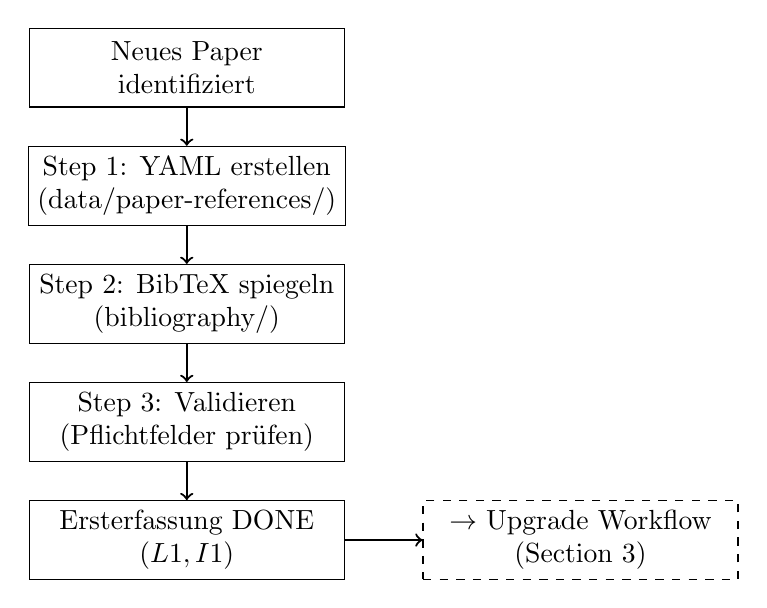
\begin{tikzpicture}[
    box/.style={rectangle, draw, minimum width=4cm, minimum height=1cm, align=center},
    arrow/.style={->, thick},
    node distance=1.5cm
]

\node[box] (new) at (0,3) {Neues Paper\\identifiziert};
\node[box] (yaml) at (0,1.5) {Step 1: YAML erstellen\\(data/paper-references/)};
\node[box] (bib) at (0,0) {Step 2: BibTeX spiegeln\\(bibliography/)};
\node[box] (valid) at (0,-1.5) {Step 3: Validieren\\(Pflichtfelder prüfen)};
\node[box] (done) at (0,-3) {Ersterfassung DONE\\$(L1, I1)$};
\node[box, dashed] (upgrade) at (5,-3) {$\rightarrow$ Upgrade Workflow\\(Section 3)};

\draw[arrow] (new) -- (yaml);
\draw[arrow] (yaml) -- (bib);
\draw[arrow] (bib) -- (valid);
\draw[arrow] (valid) -- (done);
\draw[arrow] (done) -- (upgrade);

\end{tikzpicture}
\caption{Ersterfassung Workflow: From New Paper to $(L1, I1)$}
\label{fig:ersterfassung-workflow}
\end{figure}

%%%%%%%%%%%%%%%%%%%%%%%%%%%%%%%%%%%%%%%%%%%%%%%%%%%%%%%%%%%%%%%%%%%%%%%%%%%%%%%
% SECTION 3: UPGRADE WORKFLOW
%%%%%%%%%%%%%%%%%%%%%%%%%%%%%%%%%%%%%%%%%%%%%%%%%%%%%%%%%%%%%%%%%%%%%%%%%%%%%%%

\section{The Upgrade Workflow}
\label{sec:paperint-upgrade}

\subsection{Step 0: Check Existing Content (CRITICAL)}

\textbf{Before any upgrade, check if content already exists on \texttt{origin/main}:}

\begin{verbatim}
# 1. Update remote
git fetch origin main

# 2. Check if full text exists on main
git show origin/main:papers/fulltext/PAP-xxx.txt 2>/dev/null | wc -c

# 3. If >0, checkout from main instead of fetching new
git checkout origin/main -- papers/fulltext/PAP-xxx.txt
\end{verbatim}

\begin{tcolorbox}[colback=yellow!10!white, colframe=yellow!75!black,
    title=Learning INT-L-002: Always Check Main First]
Full text often already exists on \texttt{origin/main} but is not visible on
the current branch. Always run Step 0 before attempting to fetch or create
new content.
\end{tcolorbox}

\subsection{Content Level Upgrades (Paper-Internal)}

Content upgrades focus on acquiring \textit{paper-internal information}:

\paragraph{L0 $\rightarrow$ L1 (Bibliographic $\rightarrow$ Descriptive):}
Add Abstract, Keywords, Publication Type. Source: Paper itself or DOI lookup.

\paragraph{L1 $\rightarrow$ L2 (Descriptive $\rightarrow$ Analytical):}
\label{sec:upgrade-l2}
Add Methodology, Sample Description, Key Findings, Limitations. Source: Paper's methodology section.

\paragraph{L2 $\rightarrow$ L3 (Analytical $\rightarrow$ Complete):}
Obtain full paper text including paper's own bibliography. Validate: \texttt{wc -c} must show $>$50,000 chars.

\begin{tcolorbox}[colback=yellow!5!white, colframe=yellow!75!black,
    title=MECE Reminder: Content Upgrades]
Content upgrades do \textbf{not} include parameter extraction or EBF field assignment.
Those activities belong to Integration upgrades (I1--I4).
\end{tcolorbox}

\subsection{Integration Level Upgrades (EBF-Specific)}

Integration upgrades focus on \textit{connecting the paper to EBF}:

\paragraph{I1: Classified}
Add basic EBF classification fields to BibTeX:
\begin{verbatim}
@article{PAP-xxx,
  ...
  evidence_tier = {1},
  use_for = {LIT-XXX, DOMAIN-XXX},
}
\end{verbatim}

\paragraph{I1 $\rightarrow$ I2 (Classified $\rightarrow$ Theorized):}
\label{sec:upgrade-i2}
Add theory linkages:
\begin{verbatim}
  theory_support = {MS-XX-XXX, MS-YY-YYY},
\end{verbatim}

\paragraph{I2 $\rightarrow$ I3 (Theorized $\rightarrow$ Exemplified):}
\label{sec:upgrade-i3}
Add Case Registry entry in \texttt{data/case-registry.yaml} with full 10C mapping (CAS-XXX).

\paragraph{I3 $\rightarrow$ I4 (Exemplified $\rightarrow$ Parameterized):}
Extract behavioral parameters and add to Parameter Registry (PAR-XXX):
\begin{verbatim}
  parameter = {lambda = 2.25, beta = 0.85},
\end{verbatim}
This is where $\lambda$, $\beta$, $\gamma$ values are formally captured.

\paragraph{I4 $\rightarrow$ I5 (Parameterized $\rightarrow$ Canonized):}
Add \textbf{both} Appendix Reference and Chapter Reference for full framework integration.

%%%%%%%%%%%%%%%%%%%%%%%%%%%%%%%%%%%%%%%%%%%%%%%%%%%%%%%%%%%%%%%%%%%%%%%%%%%%%%%
% SECTION 3: LEVEL 5 REQUIREMENTS
%%%%%%%%%%%%%%%%%%%%%%%%%%%%%%%%%%%%%%%%%%%%%%%%%%%%%%%%%%%%%%%%%%%%%%%%%%%%%%%

\section{Level 5: Full Integration Requirements}
\label{sec:paperint-level5}

\begin{tcolorbox}[colback=red!5!white, colframe=red!75!black,
    title=Critical: Level 5 Requires BOTH Appendix AND Chapter]
Integration Level 5 requires \textbf{two} references:
\begin{enumerate}
    \item \textbf{Appendix Reference:} Paper cited in appropriate LIT-Appendix
    \item \textbf{Chapter Reference:} Paper cited with \texttt{\textbackslash citet\{\}} in relevant chapter
\end{enumerate}
Only one of these = Level 4.5, not Level 5.
\end{tcolorbox}

\subsection{Appendix Reference}

\begin{enumerate}
    \item Identify the appropriate LIT-Appendix:
    \begin{itemize}
        \item \texttt{LIT-LEARNING}: Belief updating, advice, experience goods
        \item \texttt{LIT-FEHR}, \texttt{LIT-THALER}, etc.: Author-specific
        \item \texttt{LIT-O}: Fallback for miscellaneous papers
    \end{itemize}
    \item Add paper to Annotated Bibliography section
    \item Update \texttt{use\_for} field in BibTeX to reference the LIT-Appendix
\end{enumerate}

\subsection{Chapter Reference}

\begin{enumerate}
    \item Identify the relevant chapter based on topic:
\end{enumerate}

\begin{table}[htbp]
\centering
\caption{Chapter-Topic Mapping for Paper Citations}
\label{tab:chapter-mapping}
\begin{tabular}{@{}lll@{}}
\toprule
\textbf{Topic} & \textbf{Chapter} & \textbf{Section} \\
\midrule
Belief Updating, Advice & Ch. 11 & \S11.3 Motivated vs Informed Beliefs \\
Loss Aversion, Prospect Theory & Ch. 10 & \S10.x FEPSDE \\
Social Preferences & Ch. 7 & \S7.x Fairness \\
Time Preferences & Ch. 8 & \S8.x Temporal \\
Nudging, Defaults & Ch. 17 & \S17.x Interventions \\
Framing & Ch. 9 & \S9.x Context \\
\bottomrule
\end{tabular}
\end{table}

\begin{enumerate}
    \setcounter{enumi}{1}
    \item Use correct citation syntax:
    \begin{itemize}
        \item \texttt{\textbackslash citet\{PAP-xxx\}}: Author as subject (``Bregolin et al. (2026) show...'')
        \item \texttt{\textbackslash citep\{PAP-xxx\}}: In parentheses (``...as shown (Bregolin et al., 2026)'')
        \item \texttt{\textbackslash citealt\{PAP-xxx\}}: Without parentheses (for nested citations)
    \end{itemize}
\end{enumerate}

\subsection{Level 5 Validation}

\begin{verbatim}
# Both commands must return results:
grep -r "PAP-xxx" appendices/  # Appendix Reference
grep -r "PAP-xxx" chapters/    # Chapter Reference
\end{verbatim}

\subsection{The 6-Factor Framework for CORE Extensions}
\label{sec:paperint-6factor}

\begin{tcolorbox}[colback=blue!5!white, colframe=blue!75!black,
    title=Architecture Principle: LIT $\to$ CORE $\to$ Chapter]
\textbf{Primary Location:} LIT-Appendix (complete formalization)\\
\textbf{CORE Extension:} Only if 6-Factor Check is POSITIVE\\
\textbf{Chapter:} Cross-references only (no standalone formalization)
\end{tcolorbox}

For each relevant CORE appendix, evaluate these 6 factors:

\begin{table}[htbp]
\centering
\caption{6-Factor Decision Framework for CORE Extensions}
\label{tab:6factor-framework}
\begin{tabular}{@{}clp{7cm}c@{}}
\toprule
\textbf{F\#} & \textbf{Factor} & \textbf{Question} & \textbf{Required} \\
\midrule
F1 & Structural Novelty & Does paper introduce NEW structure (not just parameters)? & Yes \\
F2 & Axiom Contribution & Does paper require a NEW axiom in this CORE? & Recommended \\
F3 & Dimensionality Change & Does paper change the dimensionality of the CORE space? & No \\
F4 & Structure vs Parameter & Is contribution STRUCTURAL (not parametric)? & Yes \\
F5 & Universality & Does extension apply to ALL uses of this CORE? & Yes \\
F6 & New Mechanism & Does paper describe a NEW causal mechanism? & Recommended \\
\bottomrule
\end{tabular}
\end{table}

\textbf{Decision Rule:}
\begin{itemize}
    \item F1 + F4 + F5 all YES $\Rightarrow$ Extend CORE
    \item F4 = NO (parametric only) $\Rightarrow$ Add to WHERE (BBB), not CORE
    \item F5 = NO (domain-specific) $\Rightarrow$ Add to LIT or DOMAIN, not CORE
\end{itemize}

\subsection{11-Component Checklist for Level 5}
\label{sec:paperint-11components}

Level 5 (FULL) integration requires all 11 components:

\begin{enumerate}
    \item \textbf{BibTeX Entry} (\texttt{bcm\_master.bib})
    \begin{itemize}
        \item Fields: \texttt{use\_for}, \texttt{theory\_support}, \texttt{parameter}, \texttt{evidence\_tier}
        \item Also: \texttt{identification}, \texttt{external\_validity}, \texttt{notes}
    \end{itemize}

    \item \textbf{Theory Catalog} (\texttt{data/theory-catalog.yaml})
    \begin{itemize}
        \item MS-XX-XXX entry with \texttt{ebf\_restrictions}
    \end{itemize}

    \item \textbf{Case Registry} (\texttt{data/case-registry.yaml})
    \begin{itemize}
        \item CAS-XXX with 10C mapping
    \end{itemize}

    \item \textbf{Parameter Registry} (\texttt{data/parameter-registry.yaml})
    \begin{itemize}
        \item PAR-XXX-XXX with \texttt{values.literature}
    \end{itemize}

    \item \textbf{LIT Appendix} (\texttt{appendices/*LIT*.tex})
    \begin{itemize}
        \item Complete formalization with axiom (e.g., RB-7)
    \end{itemize}

    \item \textbf{CORE Extensions} (only if 6-Factor positive)
    \begin{itemize}
        \item New axiom (e.g., CMP-11, AWX-A5)
        \item Symbol table extension
        \item Cross-reference to LIT
    \end{itemize}

    \item \textbf{BCM2 Context Factors} (\texttt{data/dr-datareq/sources/context/})
    \begin{itemize}
        \item New $\Psi$-factors with \texttt{ebf\_reference}
    \end{itemize}

    \item \textbf{Chapter-Appendix Mapping} (\texttt{docs/frameworks/chapter-appendix-mapping.yaml})
    \begin{itemize}
        \item LIT-Appendix linked to relevant chapters
    \end{itemize}

    \item \textbf{Chapter Cross-References}
    \begin{itemize}
        \item HIGH: Cross-Ref Box + Appendix Reference
        \item MEDIUM: Appendix Reference only
        \item LOW: No action
    \end{itemize}

    \item \textbf{Paper YAML} (\texttt{data/paper-references/PAP-*.yaml})
    \begin{itemize}
        \item \texttt{structural\_characteristics} (S1--S6)
        \item \texttt{ebf\_integration}, \texttt{ten\_c\_mapping}
        \item \texttt{chapter\_relevance}, \texttt{key\_equations}
    \end{itemize}

    \item \textbf{Paper Full-Text Archive} (\texttt{data/paper-texts/PAP-*.md})
    \begin{itemize}
        \item Complete paper text as Markdown
    \end{itemize}
\end{enumerate}

\subsection{Chapter Relevance Analysis}
\label{sec:paperint-chapter-relevance}

Classify each chapter's relevance to determine required action:

\begin{table}[htbp]
\centering
\caption{Chapter Relevance Classification}
\label{tab:chapter-relevance}
\begin{tabular}{@{}lp{6cm}l@{}}
\toprule
\textbf{Level} & \textbf{Criteria} & \textbf{Action} \\
\midrule
HIGH & Paper extends CORE structure of chapter & Cross-Ref Box + Appendix Ref \\
MEDIUM & Paper provides evidence for chapter topic & Appendix Reference only \\
LOW & No direct structural contribution & No action required \\
\bottomrule
\end{tabular}
\end{table}

\textbf{Chapter Type Prioritization:}
\begin{itemize}
    \item \textbf{Type A (CORE):} Ch 5, 9--13 --- HIGH if CORE extended
    \item \textbf{Type B (Foundation):} Ch 1--4, 6--8 --- Usually MEDIUM (evidence)
    \item \textbf{Type C (Application):} Ch 14--24 --- HIGH if domain-applicable
\end{itemize}

\textbf{Note on CORE Chapters (9--13):} CORE extensions happen in APPENDICES, not chapters. CORE chapters automatically reference their appendices, so additional cross-references are typically not needed unless the paper adds a structural box (like the Narrative Modulation Box in Chapter 5).

\subsection{Reference Implementation and Detailed Analysis}
\label{sec:paperint-reference-impl}

\begin{tcolorbox}[colback=green!5!white, colframe=green!60!black,
    title=Reference Implementation: Bénabou, Falk \& Tirole (2018)]
\textbf{Paper:} ``Narratives, Imperatives, and Moral Reasoning'' (NBER WP 24798)

\textbf{CORE Extensions Added:}
\begin{itemize}
    \item CORE-HOW (B): CMP-11 ($\gamma$ sign reversal via narratives)
    \item CORE-WHEN (V): $\rho$ parameter (network segregation in $\Psi_S$)
    \item CORE-AWARE (AU): AWX-A5 (moral awareness modulation)
\end{itemize}

\textbf{Chapters with HIGH Relevance:} 5, 22, 23

\textbf{Full Analysis:} See \texttt{docs/workflows/level5-paper-integration-workflow.md}, Anhang A+B
\end{tcolorbox}

The detailed 6-Factor analysis for each CORE and the chapter-by-chapter relevance assessment are documented in:
\begin{itemize}
    \item \textbf{Workflow Document:} \texttt{docs/workflows/level5-paper-integration-workflow.md}
    \item \textbf{Anhang A:} Vertiefende CORE-Analyse (6-Faktoren für jeden CORE)
    \item \textbf{Anhang A.2:} Kapitel-Analyse-Matrix (HIGH/MEDIUM/LOW für alle 24 Kapitel)
    \item \textbf{Anhang A.3:} BCM2 Kontext-Faktoren Analyse
    \item \textbf{Anhang B:} Checkliste der dokumentierten Analysen
\end{itemize}

%%%%%%%%%%%%%%%%%%%%%%%%%%%%%%%%%%%%%%%%%%%%%%%%%%%%%%%%%%%%%%%%%%%%%%%%%%%%%%%
% SECTION 4: THE LEARNING LOOP
%%%%%%%%%%%%%%%%%%%%%%%%%%%%%%%%%%%%%%%%%%%%%%%%%%%%%%%%%%%%%%%%%%%%%%%%%%%%%%%

\section{The Learning Loop}
\label{sec:paperint-learning-loop}

The Learning Loop ensures continuous improvement of the integration workflow.

\begin{figure}[htbp]
\centering
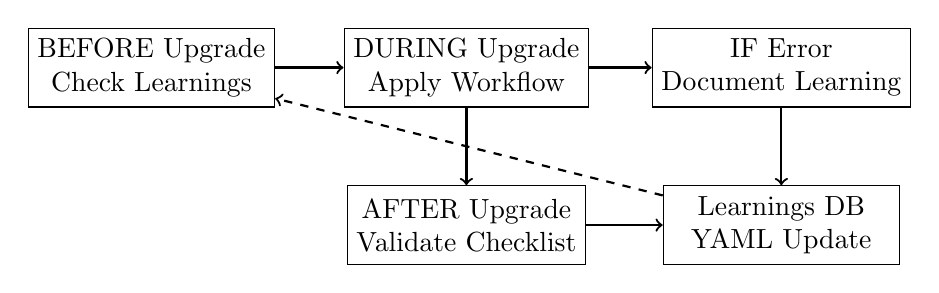
\begin{tikzpicture}[
    box/.style={rectangle, draw, minimum width=3cm, minimum height=1cm, align=center},
    arrow/.style={->, thick},
    node distance=2cm
]

\node[box] (before) at (0,2) {BEFORE Upgrade\\Check Learnings};
\node[box] (during) at (4,2) {DURING Upgrade\\Apply Workflow};
\node[box] (error) at (8,2) {IF Error\\Document Learning};
\node[box] (after) at (4,0) {AFTER Upgrade\\Validate Checklist};
\node[box] (db) at (8,0) {Learnings DB\\YAML Update};

\draw[arrow] (before) -- (during);
\draw[arrow] (during) -- (error);
\draw[arrow] (during) -- (after);
\draw[arrow] (error) -- (db);
\draw[arrow] (after) -- (db);
\draw[arrow, dashed] (db) -- (before);

\end{tikzpicture}
\caption{The Paper Integration Learning Loop}
\label{fig:learning-loop}
\end{figure}

\subsection{Step 1: Before Upgrade --- Check Learnings}

\begin{verbatim}
cat data/paper-integration-learnings.yaml | grep -A 5 "title:"
\end{verbatim}

Review known error patterns before starting.

\subsection{Step 2: During Upgrade --- Apply Workflow}

Follow the standardized workflow (Section~\ref{sec:paperint-upgrade}).

\subsection{Step 3: If Error --- Document Learning}

Add new learning to \texttt{data/paper-integration-learnings.yaml}:

\begin{verbatim}
- id: "INT-L-YYYY-MM-DD-CAT-NNN"
  date: "YYYY-MM-DD"
  category: "LEVEL|BIBTEX|LIT|THEORY|CONTENT"
  severity: "CRITICAL|HIGH|MEDIUM|LOW"
  title: "Short description"
  problem: "What happened?"
  solution: "What was the fix?"
  prevention: "How to prevent in future?"
\end{verbatim}

\subsection{Step 4: After Upgrade --- Validate Checklist}

\begin{verbatim}
☐ Content Level validated (wc -c)
☐ BibTeX syntax correct
☐ use_for field updated
☐ All cross-references bidirectional
☐ Chapter reference with correct citation syntax
\end{verbatim}

%%%%%%%%%%%%%%%%%%%%%%%%%%%%%%%%%%%%%%%%%%%%%%%%%%%%%%%%%%%%%%%%%%%%%%%%%%%%%%%
% SECTION 5: KNOWN ERROR PATTERNS
%%%%%%%%%%%%%%%%%%%%%%%%%%%%%%%%%%%%%%%%%%%%%%%%%%%%%%%%%%%%%%%%%%%%%%%%%%%%%%%

\section{Known Error Patterns}
\label{sec:paperint-errors}

\begin{table}[htbp]
\centering
\caption{Documented Error Patterns (from Learning Database)}
\label{tab:error-patterns}
\renewcommand{\arraystretch}{1.3}
\begin{tabular}{@{}llp{6cm}@{}}
\toprule
\textbf{ID} & \textbf{Category} & \textbf{Prevention} \\
\midrule
INT-L-001 & LEVEL & Validate $>$50k chars with \texttt{wc -c} \\
INT-L-002 & LEVEL & Check \texttt{origin/main} before fetching \\
INT-L-003 & LEVEL & Level 5 needs BOTH Appendix AND Chapter \\
INT-L-004 & LIT & Update \texttt{use\_for} after LIT assignment \\
INT-L-005 & BIBTEX & Use \texttt{\textbackslash citet\{\}} for subject, \texttt{\textbackslash citep\{\}} for parentheses \\
\bottomrule
\end{tabular}
\end{table}

%%%%%%%%%%%%%%%%%%%%%%%%%%%%%%%%%%%%%%%%%%%%%%%%%%%%%%%%%%%%%%%%%%%%%%%%%%%%%%%
% SECTION 6: INTEGRATION WITH EBF
%%%%%%%%%%%%%%%%%%%%%%%%%%%%%%%%%%%%%%%%%%%%%%%%%%%%%%%%%%%%%%%%%%%%%%%%%%%%%%%

\section{Integration with EBF Framework}
\label{sec:paperint-ebf-integration}

\begin{tcolorbox}[colback=yellow!5!white, colframe=yellow!75!black,
    title=Integration: METHOD-PAPERINT $\leftrightarrow$ Other Components]

\textbf{With LIT-Appendices:}
Papers at Level 5 are cited in appropriate LIT-Appendices (LIT-LEARNING, LIT-FEHR, etc.).

\textbf{With Chapters:}
Papers at Level 5 are cited in relevant chapters using \texttt{\textbackslash citet\{\}}/\texttt{\textbackslash citep\{\}}.

\textbf{With Case Registry:}
Papers at Level 3+ have corresponding CAS-XXX entries with 10C mapping.

\textbf{With Theory Catalog:}
Papers at Level 4+ are linked to MS-XX-XXX theory entries.

\textbf{With Parameter Registry:}
Papers contributing parameter estimates have PAR-XXX entries.

\textbf{With /upgrade-paper Skill:}
This appendix is the theoretical foundation for the \texttt{/upgrade-paper} Claude Code skill.

\end{tcolorbox}

%%%%%%%%%%%%%%%%%%%%%%%%%%%%%%%%%%%%%%%%%%%%%%%%%%%%%%%%%%%%%%%%%%%%%%%%%%%%%%%
% PARAMETER EXTRACTION ARCHITECTURE
%%%%%%%%%%%%%%%%%%%%%%%%%%%%%%%%%%%%%%%%%%%%%%%%%%%%%%%%%%%%%%%%%%%%%%%%%%%%%%%

\section{Parameter Extraction Architecture}
\label{sec:paperint-parameter-extraction}

This section documents the bidirectional linkage between the Paper Database
and the Parameter Registry---the ``bridge'' that transforms scientific findings
into usable behavioral parameters for EBF models.

\subsection{The Bridge Architecture}

\begin{tcolorbox}[colback=blue!5!white, colframe=blue!75!black,
    title=Parameter Extraction: Paper $\rightarrow$ Registry $\rightarrow$ Models]

\begin{verbatim}
┌─────────────────────┐     ┌─────────────────────┐     ┌─────────────────┐
│  PAPER-VOLLTEXT     │     │  PARAMETER-REGISTRY │     │  EBF-ANWENDUNG  │
│  (paper-texts/)     │     │  (parameter-        │     │  (Models, Cases,│
│                     │     │   registry.yaml)    │     │   Interventions)│
├─────────────────────┤     ├─────────────────────┤     ├─────────────────┤
│                     │     │                     │     │                 │
│  "Table IV..."      │────>│  PAR-BEH-012       │────>│  Model-Registry │
│  "α ≈ 0.85..."     │ ext │  α = 0.85          │ use │                 │
│                     │     │  source: PAP-...   │     │  Cases          │
└─────────────────────┘     └─────────────────────┘     │                 │
         ▲                          ▲                   │  Interventions  │
         │                          │                   └─────────────────┘
         │         ┌────────────────┴───────────┐
         │         │                            │
         │         │  PAPER-YAML                │
         │         │  (paper-references/)       │
         │         │                            │
         │         │  parameter_registry:       │
         └─────────│    entries: [PAR-012]     │
                   │    status: complete        │
                   └────────────────────────────┘
\end{verbatim}

\textbf{Key Insight:} The Parameter Registry is the \textit{extraction layer}---it
transforms raw paper content (tables, figures, equations) into structured,
reusable parameter values for behavioral models.

\end{tcolorbox}

\subsection{Paper-YAML Schema (4 Fields)}

Every paper with extractable parameters should have a \texttt{parameter\_registry}
block in its YAML file:

\begin{tcolorbox}[colback=green!5!white, colframe=green!75!black,
    title=Paper-YAML: parameter\_registry Schema]

\begin{verbatim}
parameter_registry:
  status: complete | partial | pending    # Extraction status
  entries:                                 # Links to PAR-IDs
    - PAR-BEH-012  # α (Disadvantageous Inequity Aversion)
    - PAR-BEH-013  # β (Advantageous Inequity Aversion)
  coverage: 1.0                            # 0.0-1.0 completeness
  extraction_date: "2026-01-31"            # When extracted
  notes: |                                 # Optional: for pending
    Paper enthält weitere Parameter...
\end{verbatim}

\textbf{Field Definitions:}
\begin{itemize}[nosep]
    \item \textbf{status}: \texttt{complete} (all parameters extracted),
          \texttt{partial} (some extracted), \texttt{pending} (none yet)
    \item \textbf{entries}: List of PAR-IDs linking to Parameter Registry
    \item \textbf{coverage}: Fraction of extractable parameters that were extracted
    \item \textbf{extraction\_date}: ISO date of last extraction
    \item \textbf{notes}: Optional documentation for pending parameters
\end{itemize}

\end{tcolorbox}

\subsection{Parameter-Registry Schema (4 Extraction Fields)}

Each parameter entry in \texttt{parameter-registry.yaml} should document
its extraction provenance:

\begin{tcolorbox}[colback=orange!5!white, colframe=orange!75!black,
    title=Parameter-Registry: extraction Schema]

\begin{verbatim}
- id: PAR-BEH-012
  symbol: α
  name: "Disadvantageous Inequity Aversion"

  values:
    literature:
      mean: 0.85
      ci_95: [0.5, 4.0]
      source: "PAP-fehr1999theory"        # ← Link to Paper

  extraction:                              # ← NEW: Provenance
    location: "Table IV, p. 844"           # Where in paper
    method: table | text | calculated      # How extracted
    confidence: high | medium | low        # Extraction certainty
    reviewed_by: null                      # Four-eyes principle

  literature_sources:
    - key: "PAP-fehr1999theory"
      finding: "α ≈ 0.85 mean, heterogeneous"
\end{verbatim}

\textbf{Extraction Field Definitions:}
\begin{itemize}[nosep]
    \item \textbf{location}: Exact location in paper (page, table, figure)
    \item \textbf{method}: How the value was obtained:
          \texttt{table} (directly from table),
          \texttt{text} (from prose),
          \texttt{calculated} (derived from reported values)
    \item \textbf{confidence}: Certainty of extraction:
          \texttt{high} (explicit value),
          \texttt{medium} (range given),
          \texttt{low} (inferred)
    \item \textbf{reviewed\_by}: Optional reviewer for quality assurance
\end{itemize}

\end{tcolorbox}

\subsection{Bidirectional Linkage}

\begin{tcolorbox}[colback=purple!5!white, colframe=purple!75!black,
    title=Bidirectional Verification]

\textbf{From Paper $\rightarrow$ Parameter:}
\begin{verbatim}
# In PAP-fehr1999theory.yaml:
parameter_registry:
  entries: [PAR-BEH-012, PAR-BEH-013]
\end{verbatim}

\textbf{From Parameter $\rightarrow$ Paper:}
\begin{verbatim}
# In parameter-registry.yaml:
- id: PAR-BEH-012
  values:
    literature:
      source: "PAP-fehr1999theory"
\end{verbatim}

\textbf{Validation Rule:} For every PAR-ID in a paper's \texttt{entries},
the corresponding parameter MUST have that paper in its \texttt{source} field.

\end{tcolorbox}

\subsection{Integration with Content Level}

Parameter extraction is an \textbf{Integration Level (I4)} activity, not a Content Level activity:

\begin{itemize}[nosep]
    \item \textbf{Content L3} = Paper full text available (prerequisite)
    \item \textbf{Integration I4} = Parameters extracted to Parameter Registry
\end{itemize}

A paper can be Content L3 (full text) but Integration I1 (no parameters extracted yet).
The \texttt{parameter\_registry.status = pending} indicates this state.

\textbf{Cross-Reference:} See Appendix BBB (CORE-WHERE) for parameter estimation
methodology and quality criteria.

%%%%%%%%%%%%%%%%%%%%%%%%%%%%%%%%%%%%%%%%%%%%%%%%%%%%%%%%%%%%%%%%%%%%%%%%%%%%%%%
% SUMMARY
%%%%%%%%%%%%%%%%%%%%%%%%%%%%%%%%%%%%%%%%%%%%%%%%%%%%%%%%%%%%%%%%%%%%%%%%%%%%%%%

\section{Summary}
\label{sec:paperint-summary}

\begin{tcolorbox}[colback=gray!5!white, colframe=gray!75!black,
    title=Appendix BM Summary: METHOD-PAPERINT (MECE-Compliant)]

\textbf{Core Contribution:}
MECE-compliant 2D Classification System for paper integration:
\begin{itemize}[nosep]
    \item \textbf{Content Level (L0--L3):} Paper-internal information
    \item \textbf{Integration Level (I1--I5):} EBF-specific linkages
\end{itemize}

\textbf{MECE Axiom (Axiom MECE-1):}
\begin{itemize}[nosep]
    \item Content = what we know \textit{about} the paper (paper facts)
    \item Integration = how paper \textit{connects} to EBF (EBF linkages)
    \item Critical: Extracted parameters ($\lambda$, $\beta$, $\gamma$) $\in$ Integration (I4), NOT Content
\end{itemize}

\textbf{Key Thresholds:}
\begin{itemize}[nosep]
    \item Content L3: $>$50,000 characters (full text)
    \item Integration I5: Appendix Reference $\land$ Chapter Reference
\end{itemize}

\textbf{Key Insights:}
\begin{itemize}[nosep]
    \item \textbf{Ersterfassung first:} Every paper starts with YAML + BibTeX $\rightarrow$ $(L1, I1)$
    \item Dimensions are \textbf{strictly orthogonal} by semantic definition
    \item Content upgrades: acquire paper facts (independent of EBF)
    \item Integration upgrades: create EBF linkages (independent of paper content)
    \item Target state: (L3, I5) = Complete + Canonized
\end{itemize}

\textbf{Operational Resources:}
\begin{itemize}[nosep]
    \item Skill: \texttt{/upgrade-paper}
    \item Workflow: \texttt{docs/workflows/paper-level-upgrade-workflow.md}
    \item Learnings: \texttt{data/paper-integration-learnings.yaml}
\end{itemize}

\end{tcolorbox}

%%%%%%%%%%%%%%%%%%%%%%%%%%%%%%%%%%%%%%%%%%%%%%%%%%%%%%%%%%%%%%%%%%%%%%%%%%%%%%%
% IMPLICATIONS
%%%%%%%%%%%%%%%%%%%%%%%%%%%%%%%%%%%%%%%%%%%%%%%%%%%%%%%%%%%%%%%%%%%%%%%%%%%%%%%

\section{Implications for Practice}
\label{sec:paperint-implications}

\subsection{For EBF Development}

\begin{itemize}
    \item \textbf{Quality Assurance:} The 2D classification ensures consistent paper quality across the framework
    \item \textbf{Reproducibility:} Standardized workflow enables any contributor to integrate papers
    \item \textbf{Continuous Improvement:} Learning Loop captures institutional knowledge
    \item \textbf{Scalability:} Clear thresholds allow batch processing of paper upgrades
\end{itemize}

\subsection{For Research Integration}

\begin{itemize}
    \item \textbf{Literature Coverage:} Systematic approach ensures comprehensive coverage
    \item \textbf{Citation Consistency:} Standardized syntax prevents compilation errors
    \item \textbf{Cross-Referencing:} Bidirectional links strengthen framework coherence
\end{itemize}

%%%%%%%%%%%%%%%%%%%%%%%%%%%%%%%%%%%%%%%%%%%%%%%%%%%%%%%%%%%%%%%%%%%%%%%%%%%%%%%
% CRITICAL FOUNDATIONS
%%%%%%%%%%%%%%%%%%%%%%%%%%%%%%%%%%%%%%%%%%%%%%%%%%%%%%%%%%%%%%%%%%%%%%%%%%%%%%%

\section{Critical Foundations}
\label{sec:paperint-foundations}

This methodology builds on the following foundational principles:

\begin{enumerate}
    \item \textbf{Ersterfassung First (Axiom ERST-1):} Every paper MUST be captured (YAML + BibTeX) before any upgrade can occur. No exceptions.
    \item \textbf{MECE Orthogonality (Axiom MECE-1):} Content and Integration are \textit{semantically} independent:
    \begin{itemize}[nosep]
        \item Content = paper-internal facts (would be relevant for any literature review)
        \item Integration = EBF-specific linkages (only relevant within EBF framework)
    \end{itemize}
    \item \textbf{Semantic Boundary:} Parameter extraction belongs to Integration, not Content
    \item \textbf{Incremental Upgrade:} Papers progress through levels sequentially
    \item \textbf{Validation Before Commitment:} All thresholds verified before claiming a level
    \item \textbf{Learning from Failure:} Errors become documented learnings
    \item \textbf{Single Source of Truth:} This appendix (BM) is authoritative for definitions
\end{enumerate}

%%%%%%%%%%%%%%%%%%%%%%%%%%%%%%%%%%%%%%%%%%%%%%%%%%%%%%%%%%%%%%%%%%%%%%%%%%%%%%%
% OPEN ISSUES
%%%%%%%%%%%%%%%%%%%%%%%%%%%%%%%%%%%%%%%%%%%%%%%%%%%%%%%%%%%%%%%%%%%%%%%%%%%%%%%

\section{Open Issues and Future Work}
\label{sec:paperint-open}

\begin{enumerate}
    \item \textbf{Automation:} Develop script to automatically detect current Content/Integration levels
    \item \textbf{Quality Metrics:} Define quantitative measures for integration quality beyond thresholds
    \item \textbf{Batch Processing:} Implement workflow for upgrading multiple papers simultaneously
    \item \textbf{Learning Analytics:} Analyze learnings database for patterns and trends
\end{enumerate}

%%%%%%%%%%%%%%%%%%%%%%%%%%%%%%%%%%%%%%%%%%%%%%%%%%%%%%%%%%%%%%%%%%%%%%%%%%%%%%%
% GLOSSARY
%%%%%%%%%%%%%%%%%%%%%%%%%%%%%%%%%%%%%%%%%%%%%%%%%%%%%%%%%%%%%%%%%%%%%%%%%%%%%%%

\section{Glossary of Terms}

\begin{tabular}{@{}lp{8cm}@{}}
\toprule
\textbf{Term} & \textbf{Definition} \\
\midrule
Content Level (L0--L3) & Measure of paper-internal information depth (Bibliographic $\rightarrow$ Complete) \\
Integration Level (I1--I5) & Measure of EBF-specific linkage depth (Classified $\rightarrow$ Canonized) \\
MECE & Mutually Exclusive, Collectively Exhaustive (orthogonality principle) \\
Paper-Internal & Information from the paper itself, independent of EBF \\
EBF-Specific & Linkages and classifications unique to EBF framework \\
Parameterized (I4) & Integration level where behavioral parameters are extracted \\
Learning Loop & Continuous improvement mechanism via documented lessons \\
LIT-Appendix & Literature review appendix (LIT-FEHR, LIT-THALER, etc.) \\
EBF Fields & BibTeX fields specific to EBF (use\_for, theory\_support, parameter, etc.) \\
\bottomrule
\end{tabular}

\vspace{1em}
\textit{For complete symbol definitions, see Appendix GLS (Central Glossary).}

%%%%%%%%%%%%%%%%%%%%%%%%%%%%%%%%%%%%%%%%%%%%%%%%%%%%%%%%%%%%%%%%%%%%%%%%%%%%%%%
% REFERENCES
%%%%%%%%%%%%%%%%%%%%%%%%%%%%%%%%%%%%%%%%%%%%%%%%%%%%%%%%%%%%%%%%%%%%%%%%%%%%%%%

\section{References}
\label{sec:paperint-references}

\subsection{Cross-References}

\begin{itemize}
    \item \textbf{Appendix GLS:} Central Glossary for term definitions
    \item \textbf{Appendix CAS:} Case Registry schema and structure
    \item \textbf{Appendix MS:} Theory Catalog and MS-XX-XXX format
    \item \textbf{LIT-* Appendices:} Literature reviews (LIT-FEHR, LIT-THALER, LIT-LEARNING, etc.)
    \item \textbf{Appendix BBB:} Parameter Registry for PAR-XXX entries
\end{itemize}

\subsection{Operational Resources}

\begin{itemize}
    \item \textbf{Skill:} \texttt{/upgrade-paper} (Claude Code)
    \item \textbf{Workflow Documentation:} \texttt{docs/workflows/paper-level-upgrade-workflow.md}
    \item \textbf{Learning Database:} \texttt{data/paper-integration-learnings.yaml}
    \item \textbf{Master Bibliography:} \texttt{bibliography/bcm\_master.bib}
\end{itemize}

\subsection{Key Literature}

This methodology appendix is primarily operational and does not directly reference
external literature. For relevant behavioral economics papers, see the LIT-* appendices
and the master bibliography.

\nocite{bcm_master}

% =============================================================================
% END OF APPENDIX BM
% =============================================================================
